\chapter{
  High Granularity Calorimeter Upgrade
 }\label{ch_hgcal}

By the start of the Run4 period of proton-proton collisions
at \gls{LHC}, the collision energy is expected to
reach its full design limit of 14 \TeV{} and
commissioning of \gls{HL-LHC} is expected to
increase the luminosity by \(~10\) times.
The integrated luminosity collected by the end of Run5 (2038)
is expected to be 3000 \fbinv{}.

With increased luminosity, the \gls{CMS} detector will get
higher dose of radiation and the average number of pileup interactions
will be of the order \( O(140) \). The endcap calorimeters \gls{ECAL} and \gls{HCAL} will suffer
irreparable damage due to the much higher radiation dose received
from the increased luminosity in those regions.
The \gls{HGCAL} is an upgrade that will replace current endcap calorimeters
(\gls{ECAL} and \gls{HCAL}).
\gls{HGCAL} is expected to be completed and installed
during \gls{LS3} (2026--2028).

This chapter will discuss broadly the design
of \gls{HGCAL}, especially its scintillator section with
studies done at \gls{NICADD} towards its upgrade.
For complete design see the \gls{TDR}~\cite{cms-hgcal-tdr}.

\section{
  Technical Design and Requirements
 }\label{ch_hgcal:technical-design}

As mentioned, the \gls{HGCAL} will replace current endcap \gls{ECAL} and
\gls{HCAL}. Figure~\ref{fig:cms-hgcal-quadrant-layout}
shows exactly where the new detector will be placed. The image on the right in
Figure~\ref{fig:cms-hgcal-quadrant-layout} shows a side view (\( z-r \) plane)
of the detector. Starting from the left i.e.~innermost layers is the
\gls{CE-E} whose active layers are made of silicon cells
(\( \approx 0.5-1 \cm{}^2\)). The
majority of the detector in longitudinal depth is \gls{CE-H}
whose starting few active layers are also all silicon followed
by mixed layers with silicon cells in lower rings of the
layer and scintillator tiles (\( \approx 5-31 \cm{}^2\)) in the rest.
Silicon is radiation hard material i.e.~the response of silicon cells
will be adequate under accumulated radiation dose over time. But
silicon is also expensive and for such high coverage area in \gls{HGCAL},
it significantly increases the construction cost of the project. For this
reason scintillator tiles are used wherever radiation doses are low
enough as they offer good performance at reasonable cost.
Some of the main reasons for high cell count, lateral and longitudinal granularity
are to preserve energy resolution after 3000 \fbinv{}, aid \glsfirst{PF}
reconstruction in rejecting energy deposit from pileup using precise timing measurement, and
being able to observe narrower jets with \( R = 0.2 \).
To be able to deliver these requirements both silicon cells and scintillator tiles
need to have good \gls{SNR} even after 3000 \fbinv{}.

\begin{figure}[!ht]
  \centering
  \begin{minipage}[c]{0.49\textwidth}
    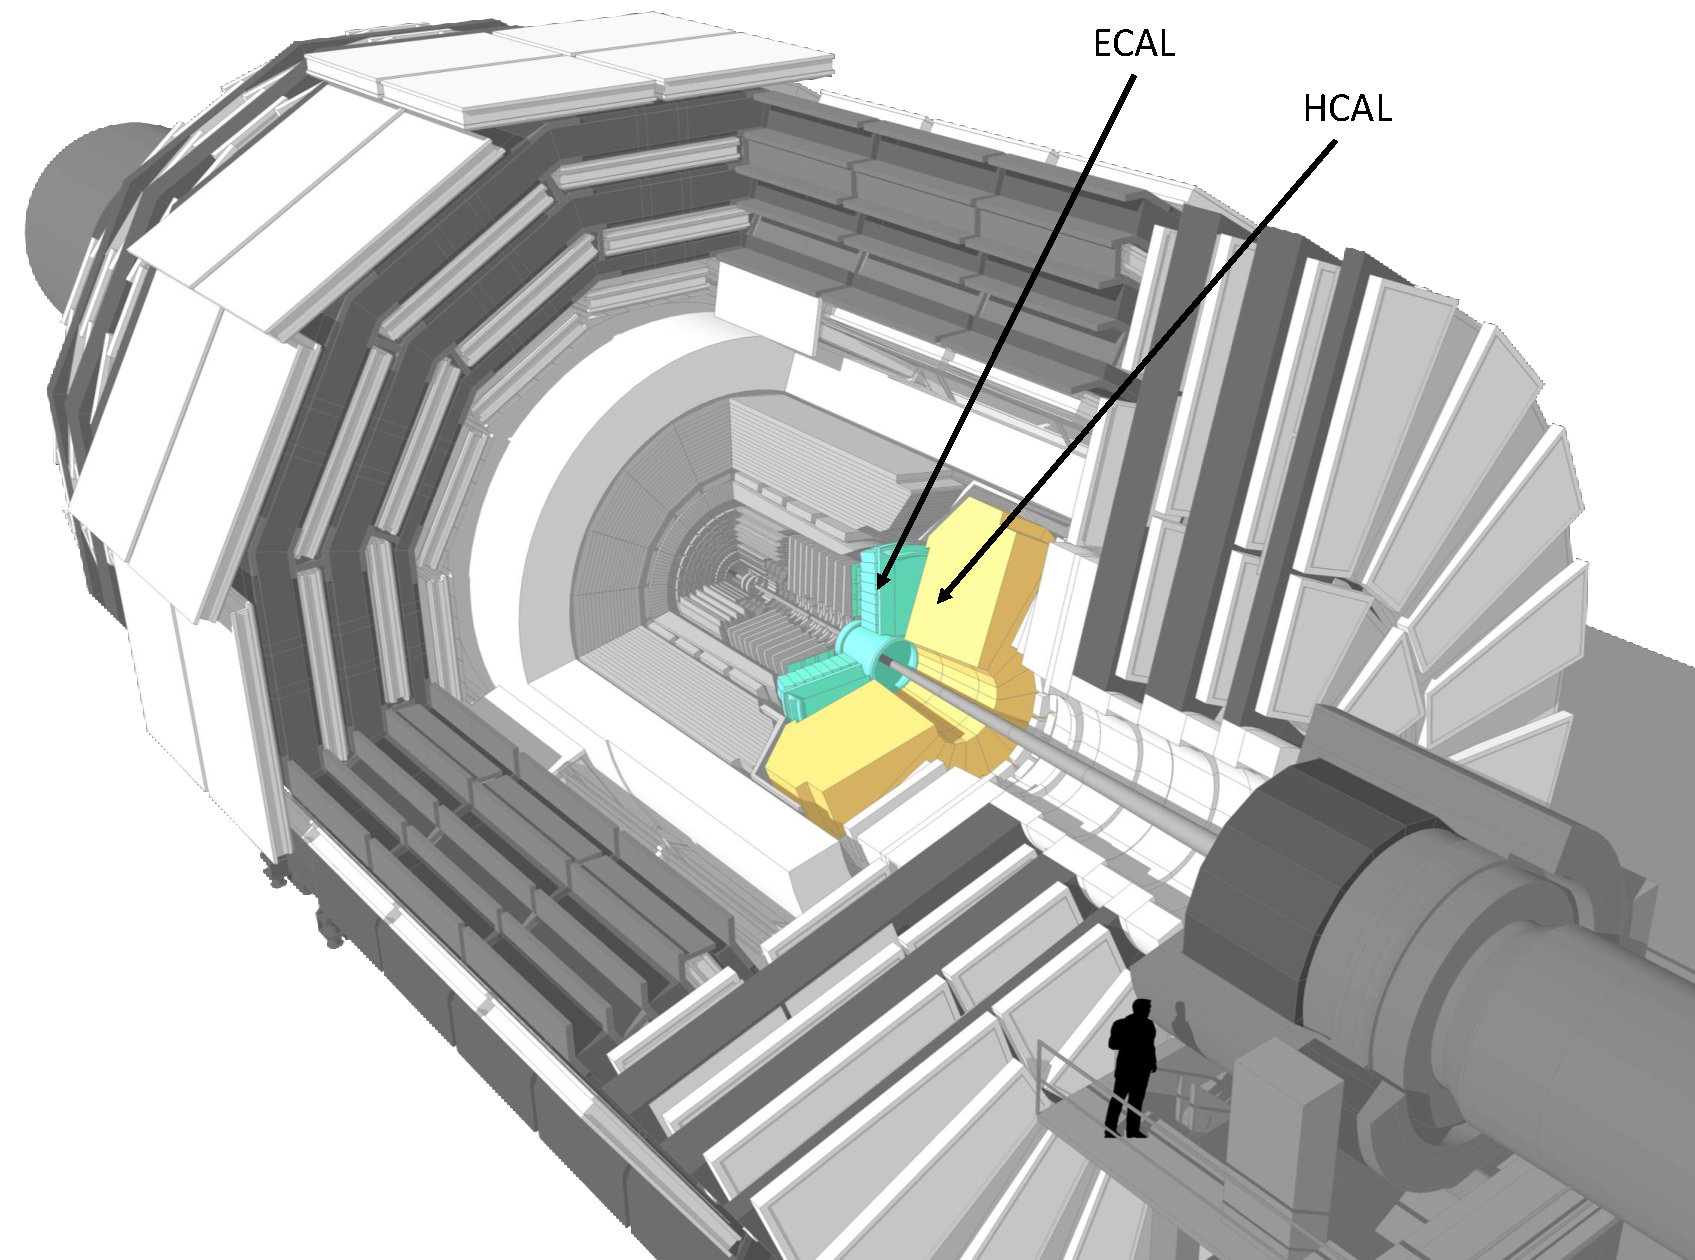
\includegraphics[width=\textwidth]{figures/hgcal/hgcal_place.pdf}
  \end{minipage}
  \begin{minipage}[c]{0.49\textwidth}
    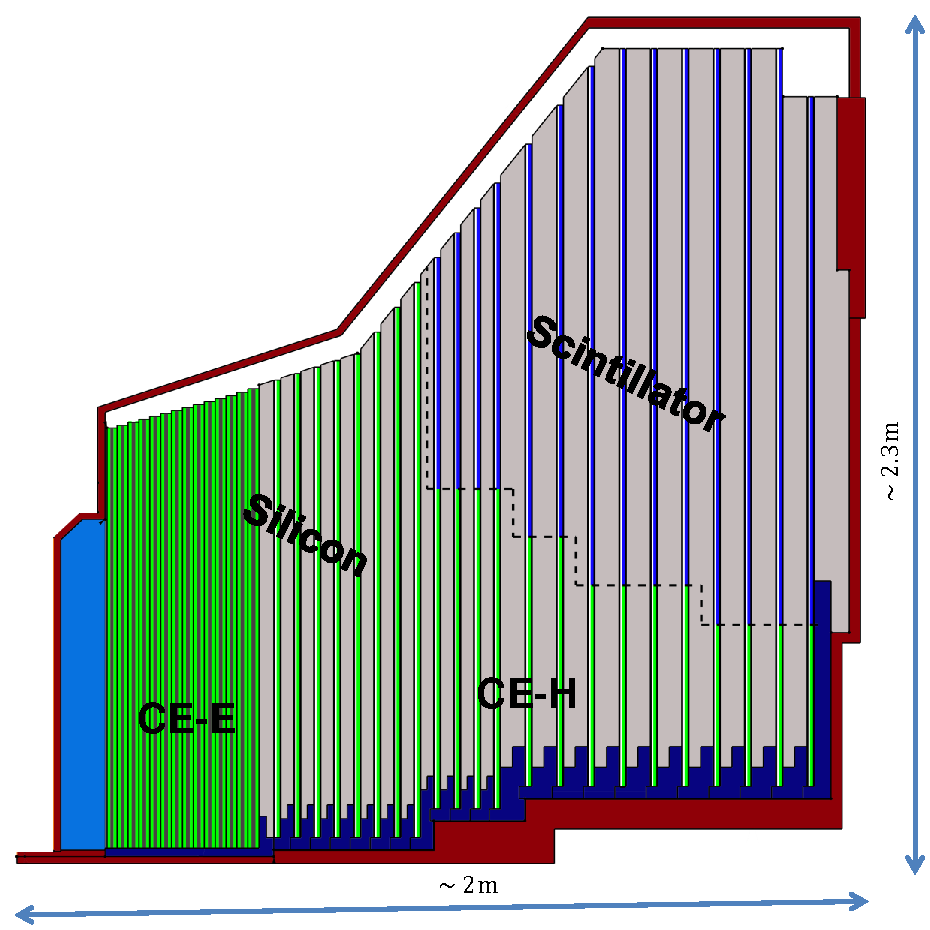
\includegraphics[width=0.9\textwidth]{figures/hgcal/hgcal_quadrant.pdf}
  \end{minipage}
  \caption[Overview of HGCAL position and quadrant view of CE]%
  {Overview of HGCAL position and quadrant view of \gls{CE}. Left image
    shows current endcap \gls{ECAL} and \gls{HCAL} highlighted.
    Right image shows quadrant view of \gls{HGCAL} from the side~\cite{image-cms-hgcal-quadrant-layout,image-cms-hgcal-place}.}%
  \label{fig:cms-hgcal-quadrant-layout}
\end{figure}

\clearpage
\section{
  Scintillator Tiles and SiPMs
 }

Silicon cells will be directly fabricated 8 inch silicon wafers (432
cells) (shown
in Figure~\ref{fig:hgcal-layer-22} as yellow and green colored hexagons),
whereas each scintillator tile will need to be prepared separately
and assembled in the form of a ``tileboard'' (about \(8\times 8\) tiles).
Figure~\ref{fig:hgcal-layer-22} shows scintillator
tile boundary with red grid lines. There are 288
scintillator tiles in
each ring, and each layer has different
number of rings of scintillator tiles with a maximum of 42 rings. To reduce
the production cost and assembly complexities, scintillator sizes are
same for every two rings. The ring number is used to identify tile
size, for example R18--19 (Figure~\ref{fig:hgcal-scintillator-tile}) is the size of tiles in ring number 18 and 19.

\begin{figure}[!ht]
  \centering
  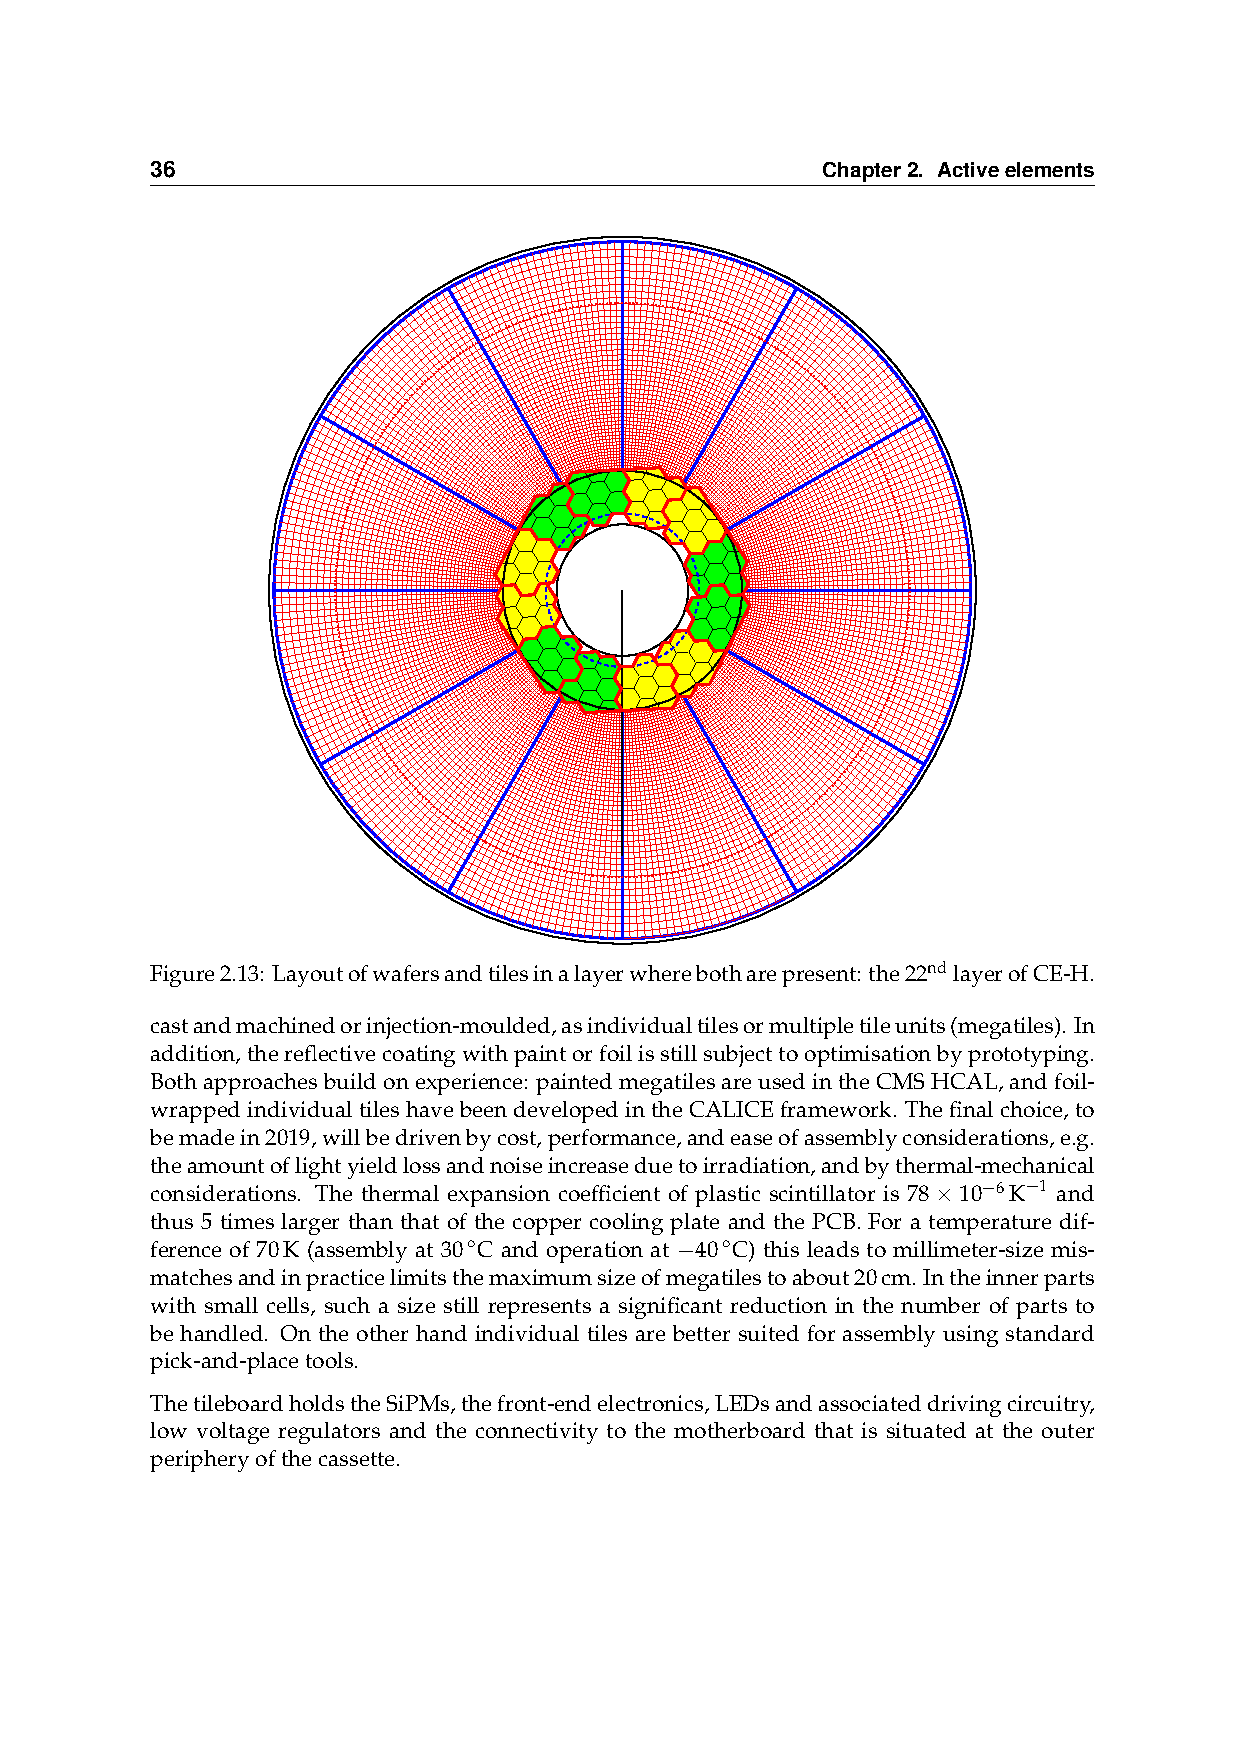
\includegraphics[trim={129 389 127 113},clip,width=0.5\textwidth]{figures/hgcal/page36_TDR_HGCAL.pdf}
  \caption[CE-H mixed layer 22]
  {CE-H mixed layer 22. This is the last layer
    in CE-H (Right image Figure~\ref{fig:cms-hgcal-quadrant-layout}).
    Yellow and green hexagons are the
    8 inch silicon modules and the red grid lines shows
    11,520 (40 rings) scintillator tiles.~\cite{cms-hgcal-tdr}.}%
  \label{fig:hgcal-layer-22}
\end{figure}

\subsection{
  Scintillator Materials
}

Materials which scintillate i.e.~emits light
whenever ionizing radiation passes through it are known as
scintillators. Scintillators can be crystals (current barrel and endcap
\gls{ECAL}), liquid or plastic and are broadly divided into two
categories organic or inorganic.
\gls{HGCAL} will make use of organic plastic scintillator. The most
commonly used base material in scintillators of this type are \gls{PVT} and \gls{PST}.
\gls{PVT} and \gls{PST} are base material and
by themselves cannot serve as scintillators for a couple of
reasons. The light emitted is at lower wavelengths (ultraviolet)
and they are barely transparent to this light.
For these reasons they have a small percentage of dopants added
which absorb the scintillation light and re-emit it at larger wavelengths (visible).
A second dopant is added to further increase the attenuation length of
the light emitted, so that light can be collected and coupled to a light
detection system.

The plastic scintillator can be produced via extrusion, casting or injection molding.
\gls{PVT} and \gls{PST} are used as base material for the cast and
injection molded scintillator tiles, respectively.

Cast scintillators are generally brighter (in terms of light output)
than injection molded scintillators, but the production cost of
cast scintillator per unit area is generally higher and additional
machining costs.
Choice of scintillator in addition to \gls{SiPM}, which will be discussed next,
impacts the cost-performance optimization.

\subsection{
  SiPMs
}

\gls{SiPM} is a solid-state device that converts incident photons to electric
current with a large gain (\( 10^5 \) to \( 10^6 \)).
\glspl{SiPM} achieve this with pixels (10\micron{} to 100\micron{} in size)
connected in parallel, where each pixel is an avalanche photodiode (APD)
combined with quenching resistor. For example a \gls{SiPM} of active
area \( 2\mm{}^2 \) with 15\micron{} pixel has approximately 9,000 pixels.
Commercially \glspl{SiPM} produced by Hamamatsu Photonics are also known as \gls{MPPC}~\cite{mppc-13360}. Figure~\ref{fig:hgcal-sipm}
shows \gls{SiPM} next to tip of a pen.

\gls{SiPM} operates in reverse bias (Geiger Mode) with \gls{OV} above \gls{BR}.
It has a linear relationship between \(V\)(\(= V_{\texttt{O}} - V_{\texttt{BR}} \)) and the gain.
In addition to low operating voltage (\(40-60\) V) the power
consumption is also low.
For \gls{HGCAL} Hamamatsu S14160~\cite{mppc-14160} is being considered with
active area 2, 4 and \(9\mm{}^2\). Larger area means larger signal, but
also higher intrinsic noise and power consumption.

For \gls{HGCAL} the \glspl{SiPM} will be mounted on \gls{PCB},
and prepared scintillator tiles will be directly glued
over the \glspl{SiPM} with the dimple centered on the \gls{SiPM}'s active area.

\begin{figure}[!ht]
  \centering
  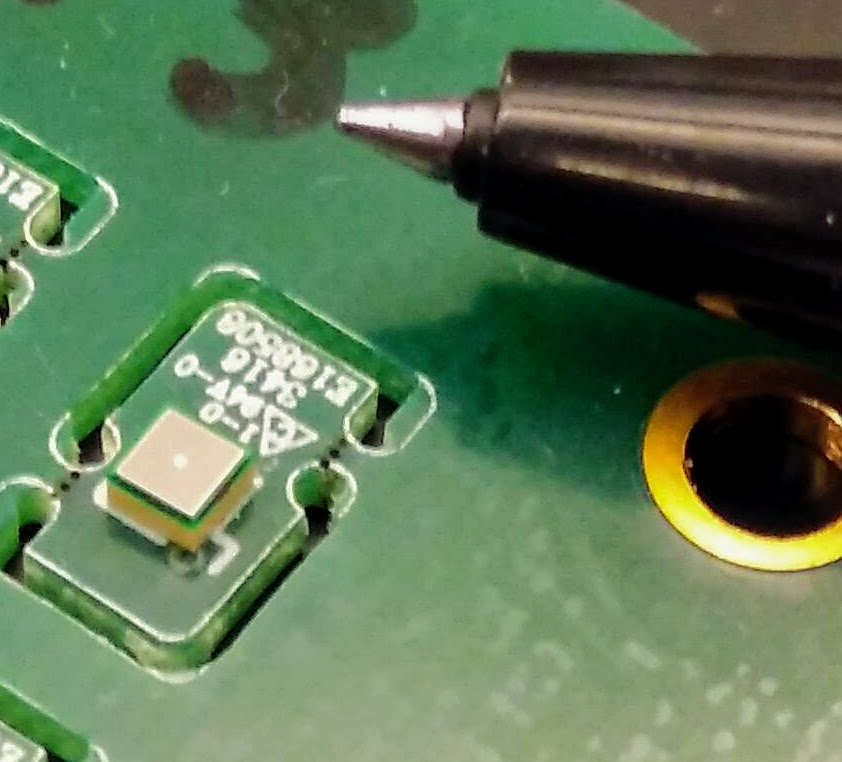
\includegraphics[width=0.4\textwidth]{figures/hgcal/sipm.jpg}
  \caption[SiPM]{SiPM}%
  \label{fig:hgcal-sipm}
\end{figure}

\subsection{
  Scintillator Tiles
}\label{ch_hgcal:scint-tiles}

Scintillator tiles coupled directly to \glspl{SiPM} alone cannot provide
sufficient response to the \glsfirstplural{MIP}.
Additionally
the response will be non-uniform at the \gls{SiPM}. Higher
signal and uniformity of response, can be achieved by either coating or wrapping the tile in reflective
material~\cite{niu-sipm-on-tile}. \gls{ESR}
is a multi-layer highly reflective material with 65\micron{} thickness (Figure~\ref{fig:hgcal-esr-wrapper}), is the material chosen for wrapping the scintillator tiles.

To wrap 239,616 individual tiles  with \gls{ESR} is a very challenging task.
At NIU we have built an automated wrapping machine (Section~\ref{ch_hgcal:wrapping}) to
wrap scintillator tiles with speed and repeatability.

\begin{figure}[!ht]
  \centering
  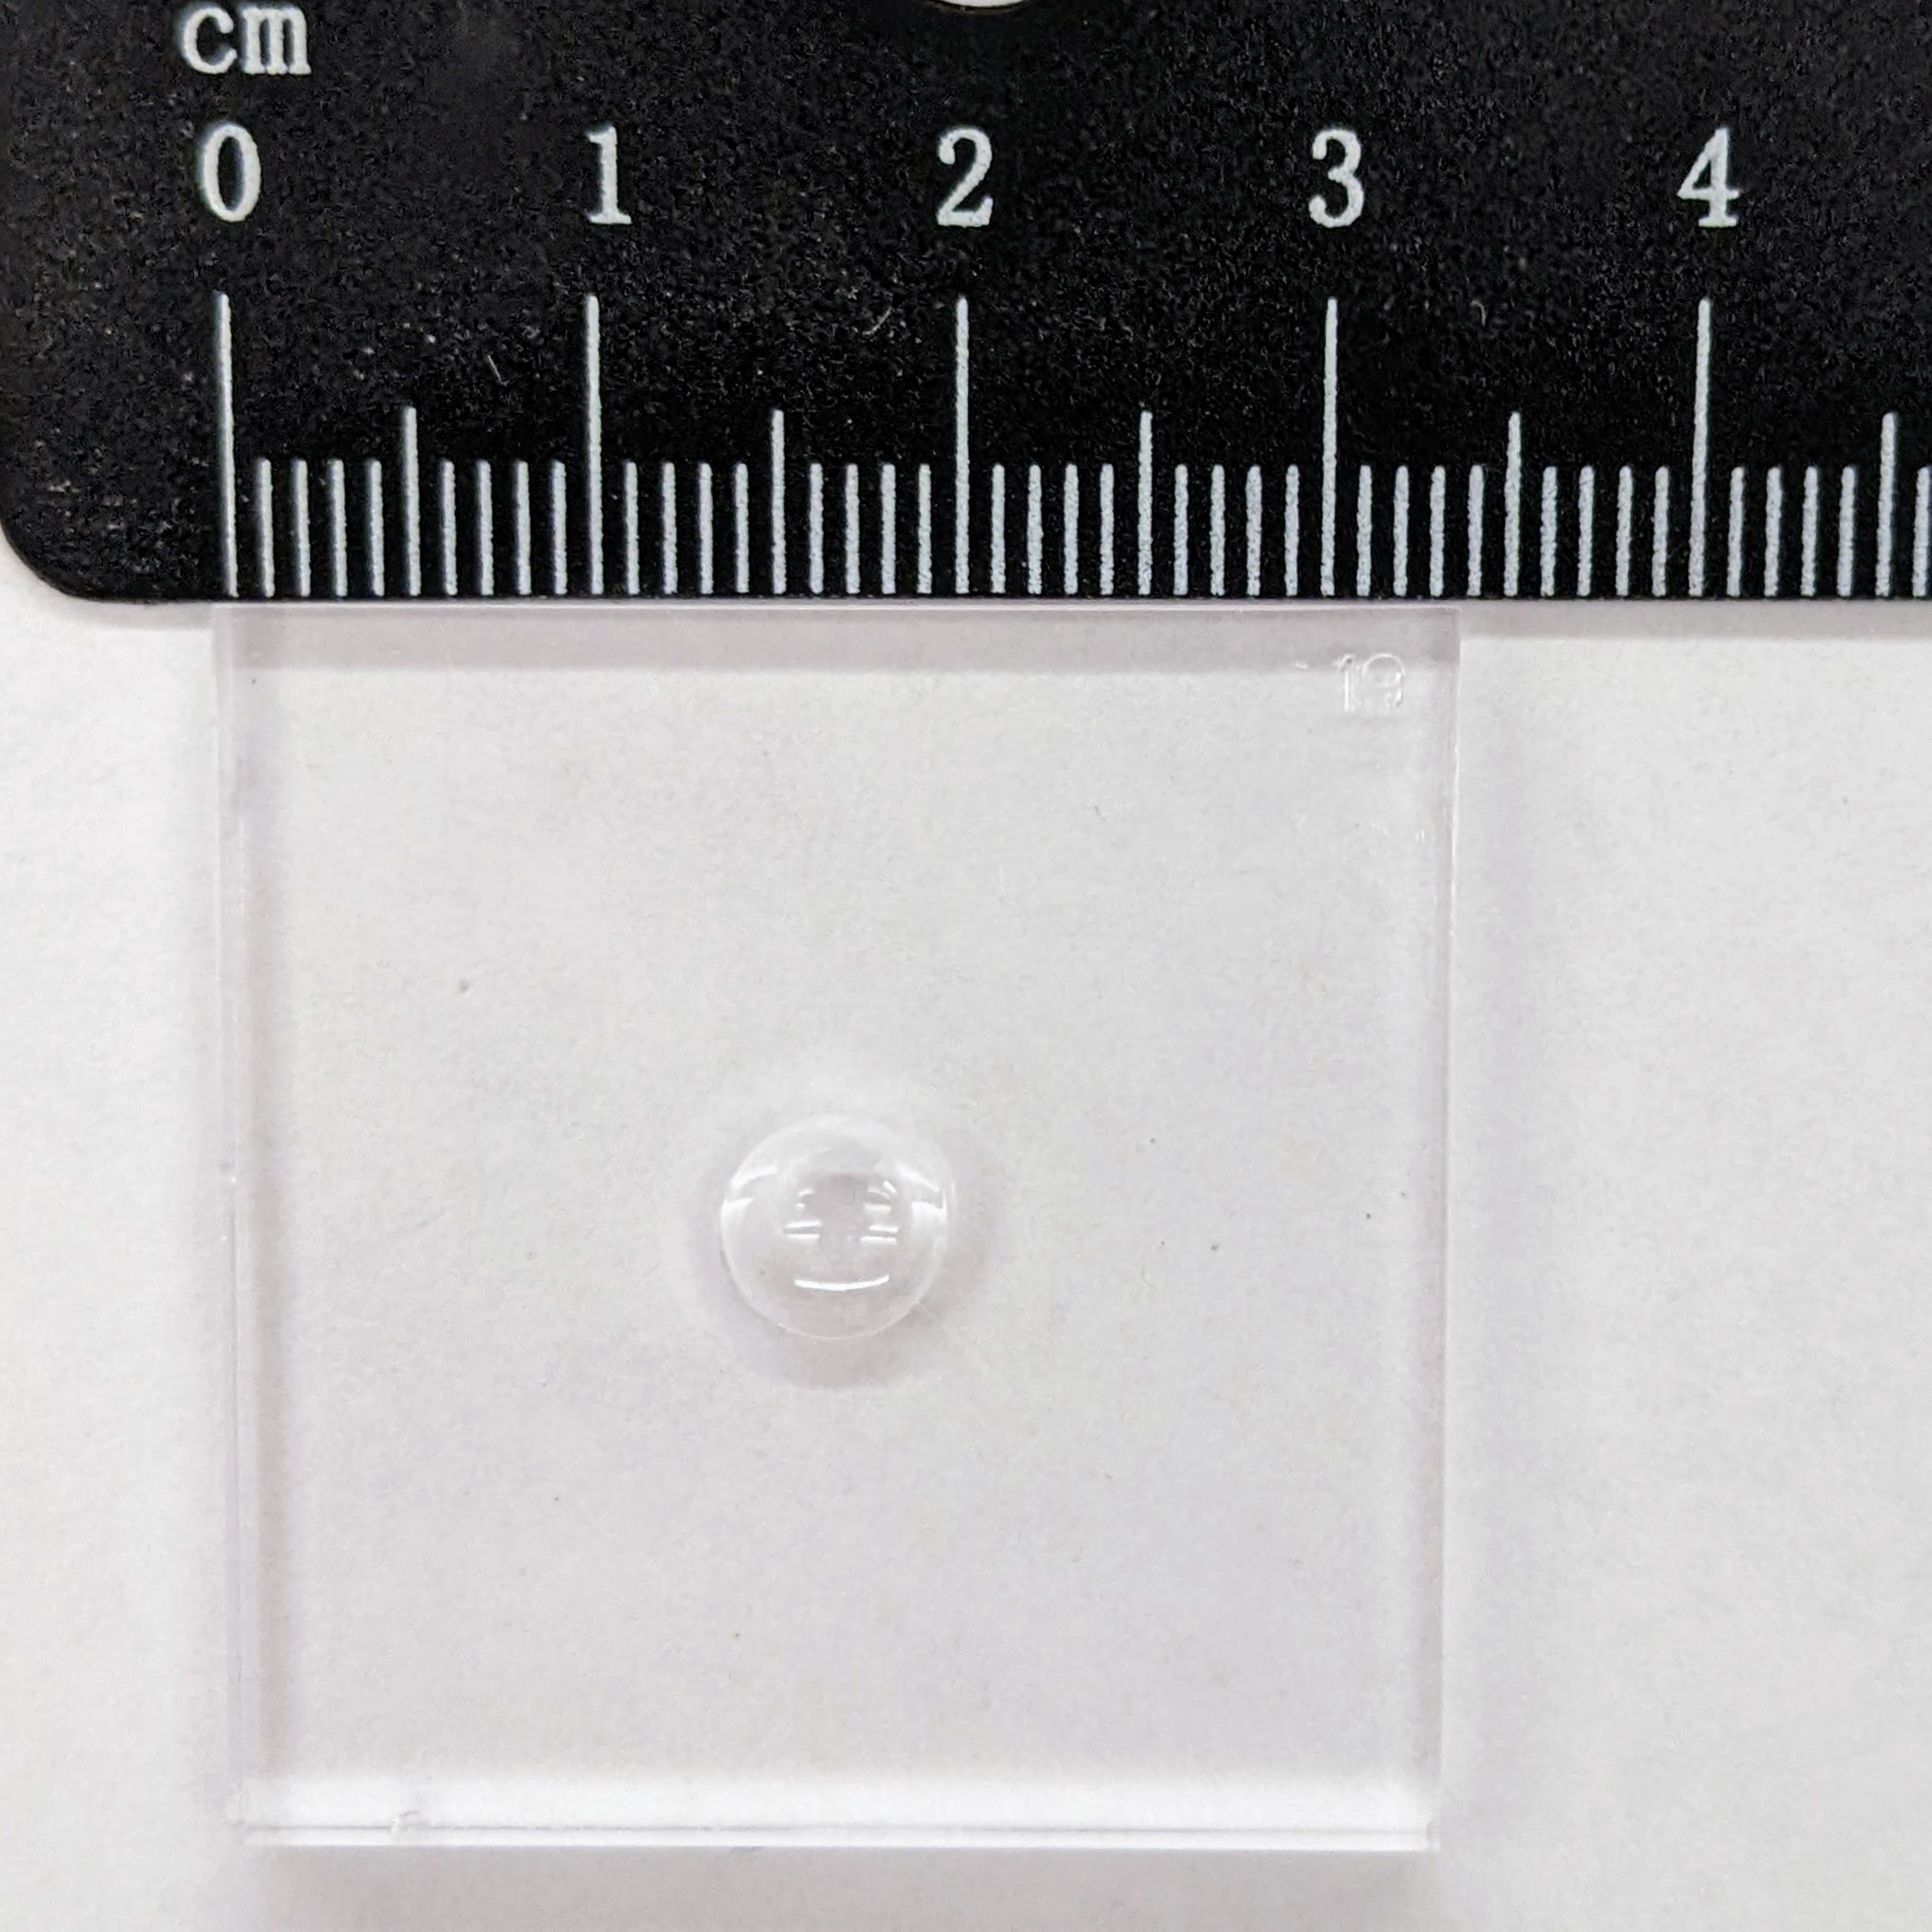
\includegraphics[width=0.5\textwidth]{figures/hgcal/tile_19.jpg}
  \caption[Scintillator tile with dimple]{Scintillator tile with dimple}%
  \label{fig:hgcal-scintillator-tile}
\end{figure}

\begin{figure}[!ht]
  \centering
  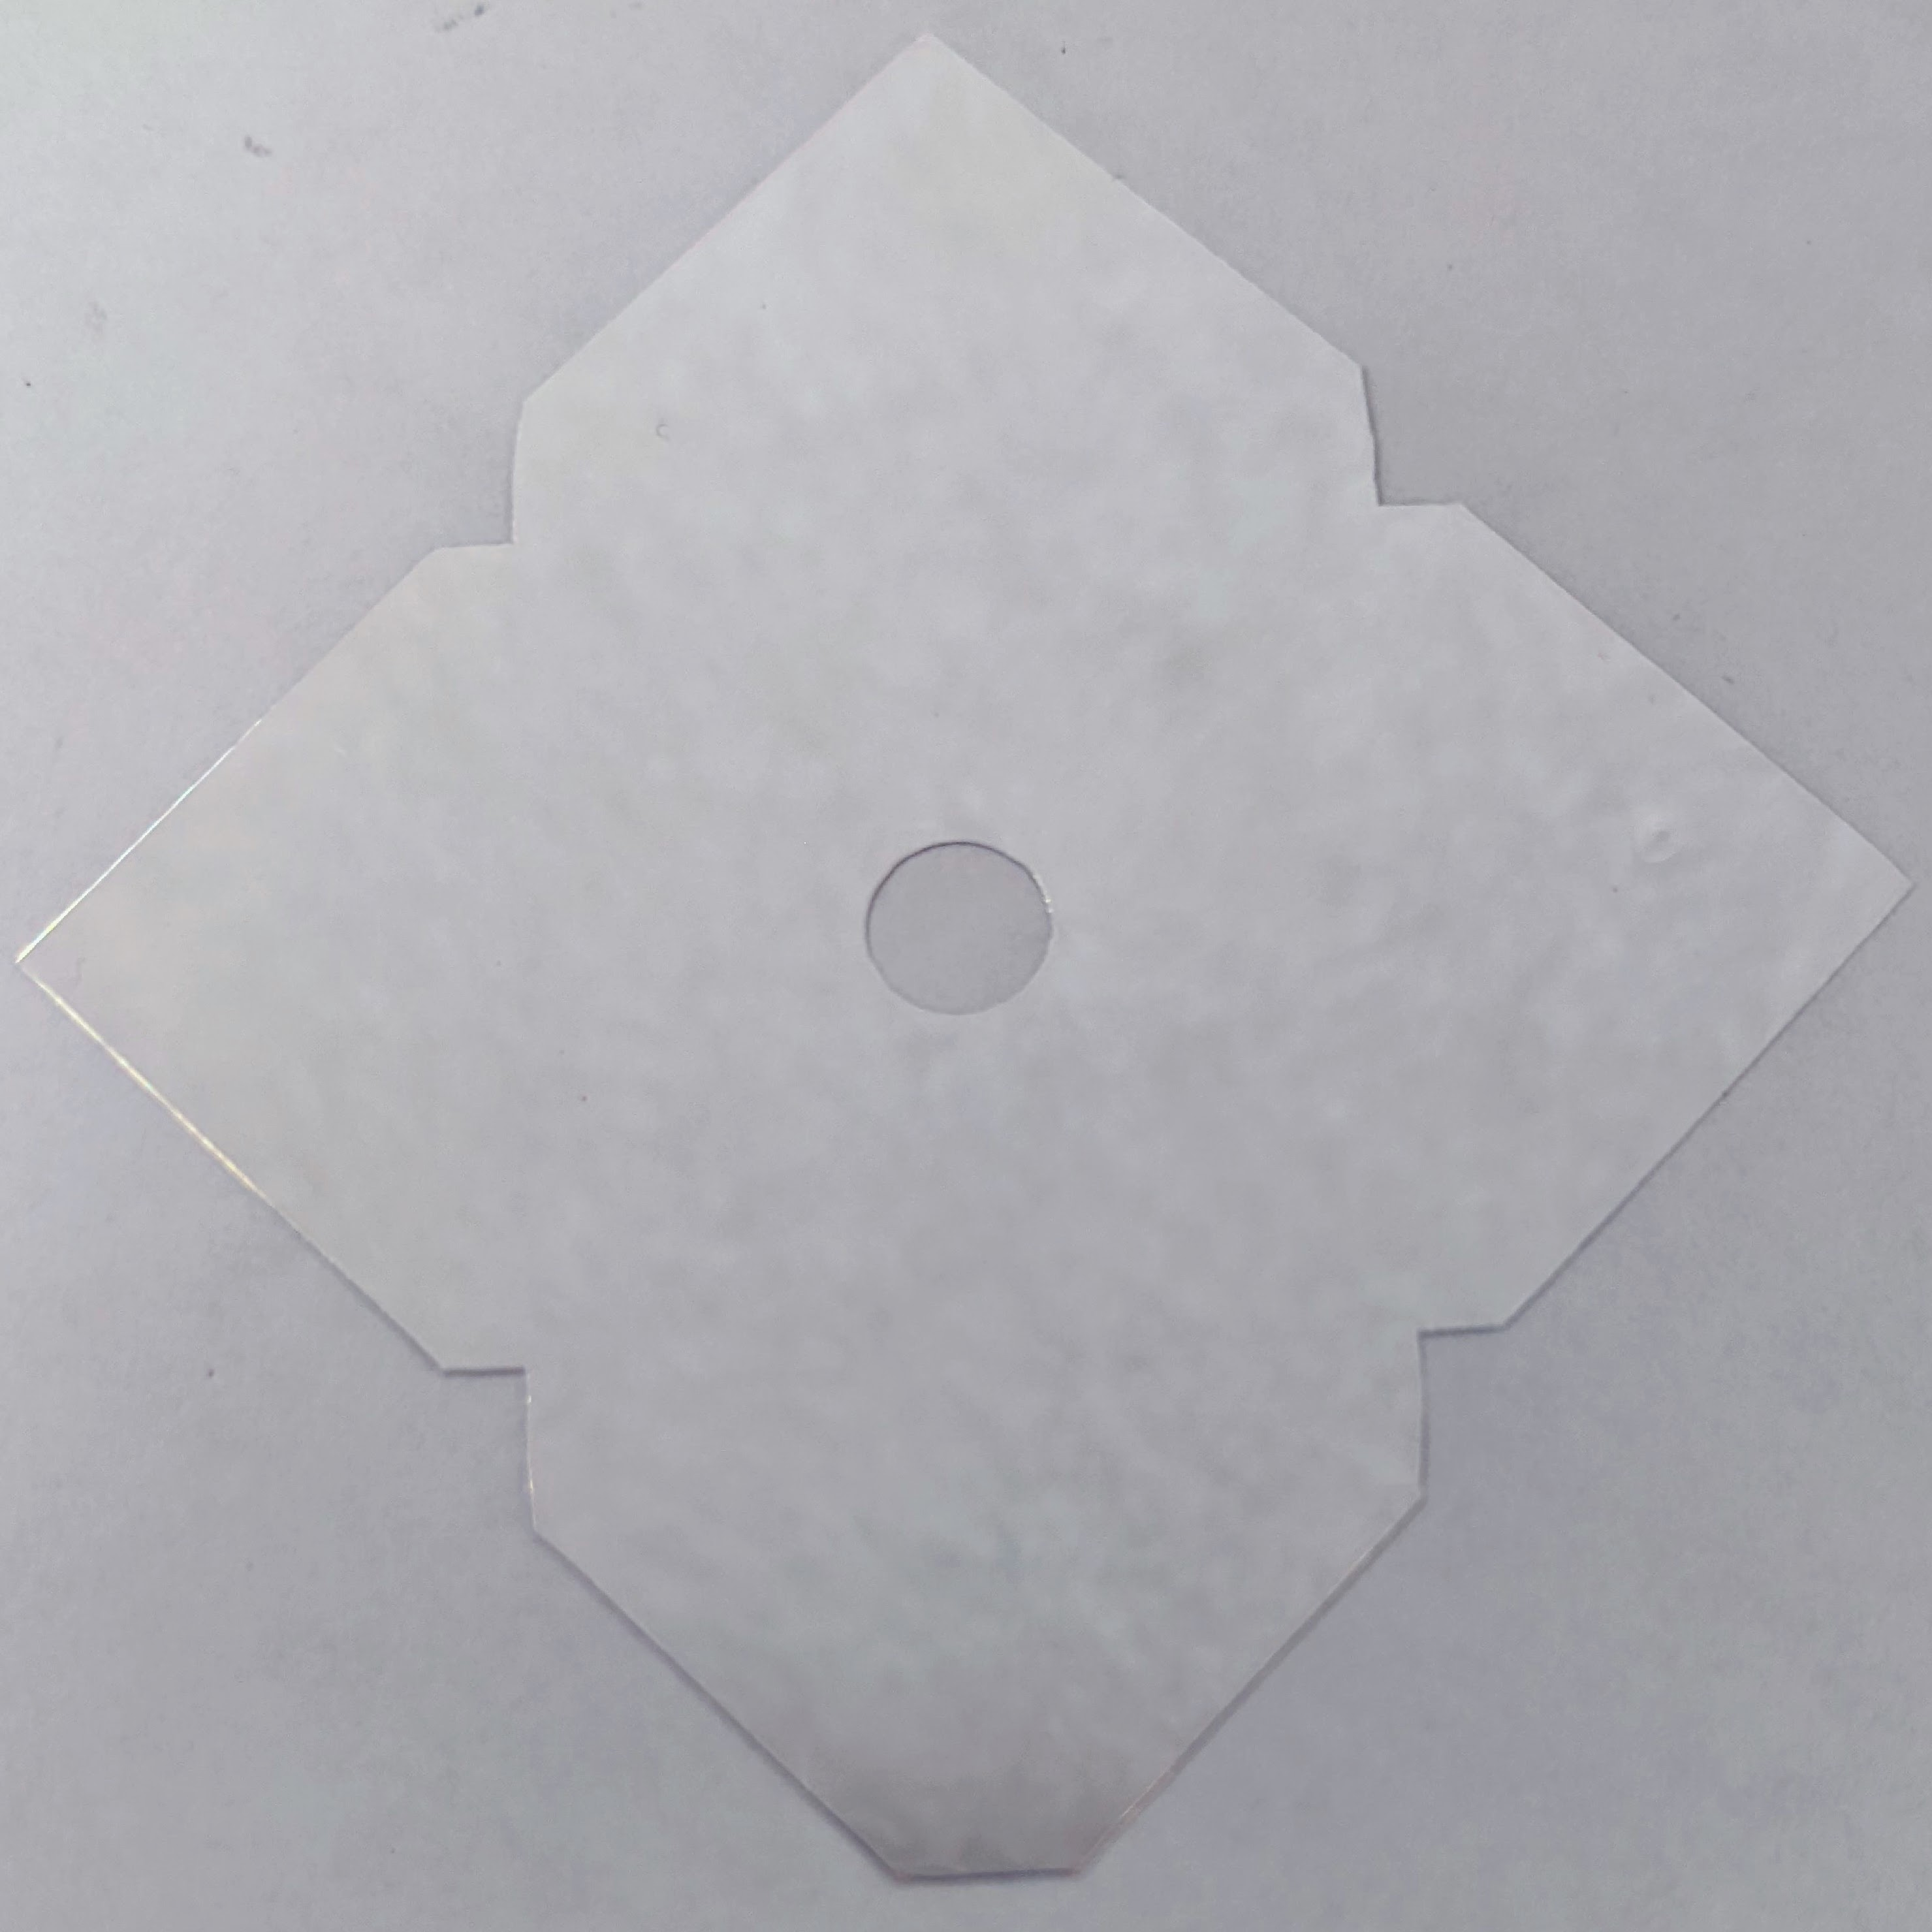
\includegraphics[width=0.5\textwidth]{figures/hgcal/esr_wrapper.jpg}
  \caption[ESR wrapper cut for tile size R18--19]
  {ESR wrapper cut for tile size R18--19}%
  \label{fig:hgcal-esr-wrapper}
\end{figure}

The final wrapped tile in complete automated process
with wrapping machine built at NIU
is shown in Figure~\ref{fig:hgcal-scintillator-tile-wrapped}.

\begin{figure}[!ht]
  \centering
  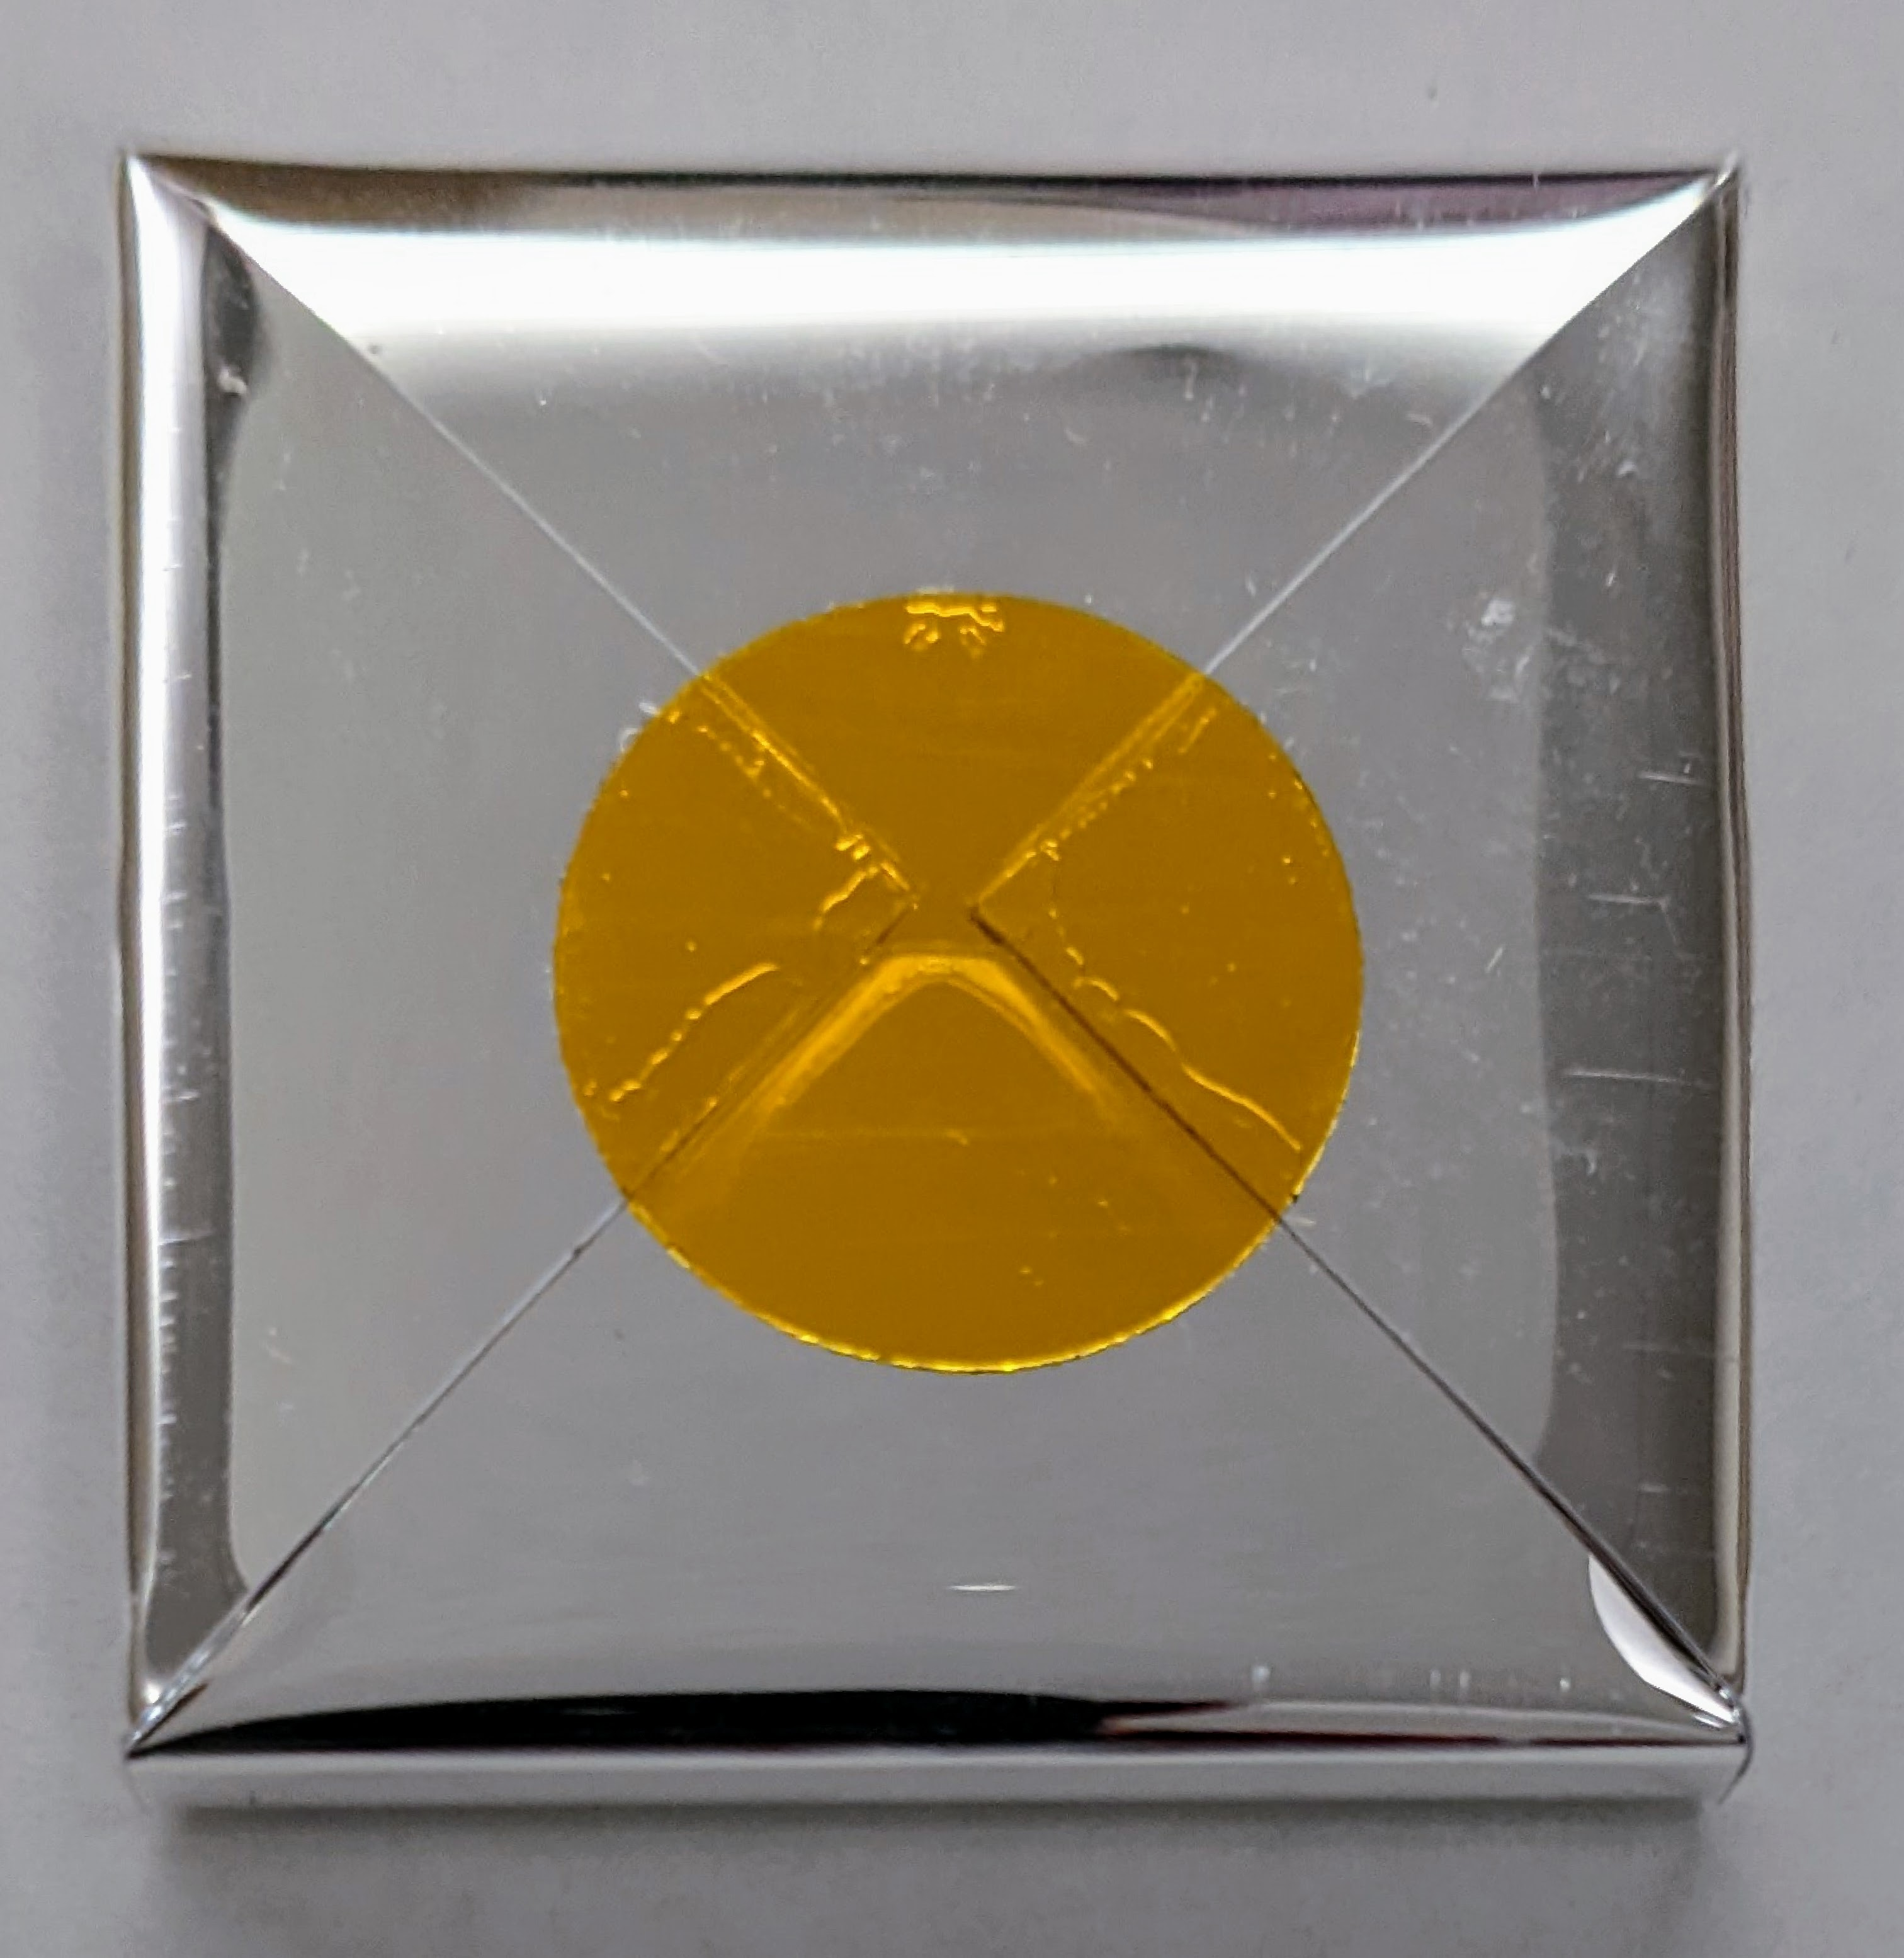
\includegraphics[width=0.4\textwidth]{figures/hgcal/wrapped_tile_up.jpg}
  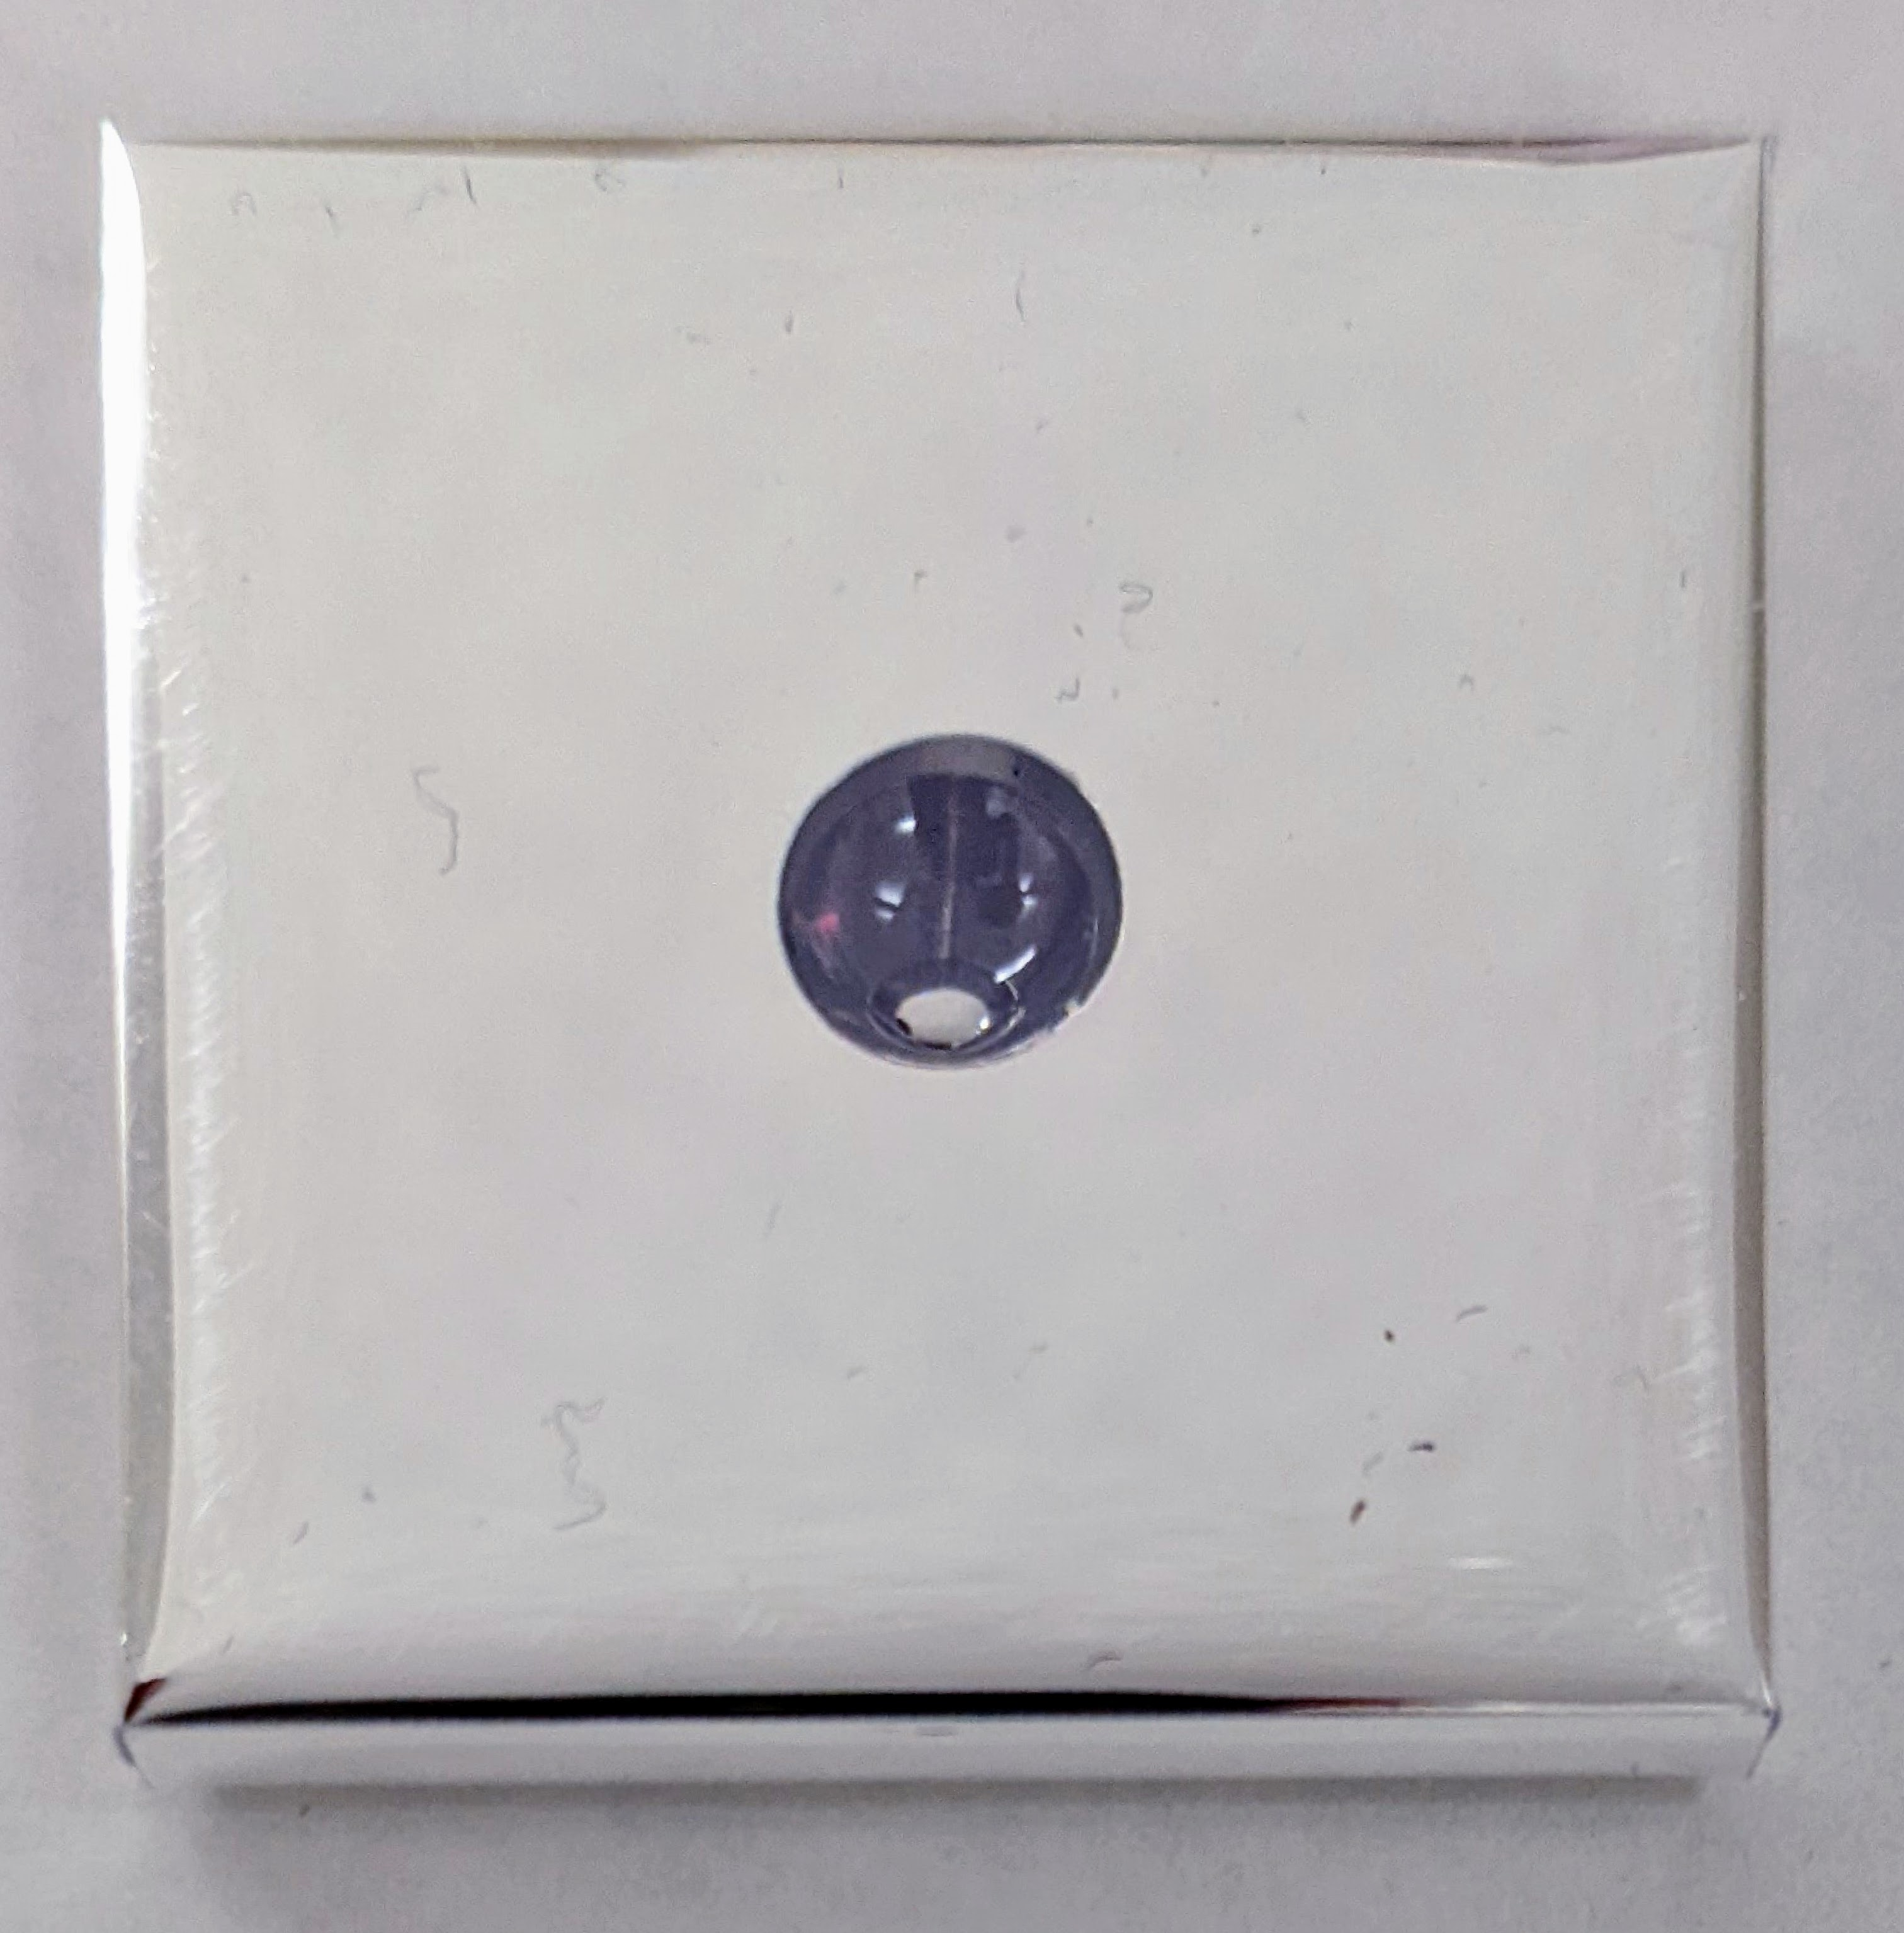
\includegraphics[width=0.4\textwidth]{figures/hgcal/wrapped_tile_down.jpg}
  \caption[R18--19 scintillator tile wrapped in ESR]
  {R18--19 scintillator tile wrapped in ESR\@. Left: Upside of the tile, with
    Kapton sticker holding the flaps. Right: Bottom side with center hole
    over dimple.}%
  \label{fig:hgcal-scintillator-tile-wrapped}
\end{figure}

\clearpage
\section{
  Automated Wrapping of Scintillator Tiles
 }\label{ch_hgcal:wrapping}

As mentioned in Section~\ref{ch_hgcal:scint-tiles}, the number
of wrapped scintillator tiles required for the \gls{HGCAL}
is very large, 239,616 tiles. In addition to the large number
of tiles, the tiles will be of different sizes and repeatability
in wrapped tile quality is required for reliable performance
of the detector. Figure~\ref{fig:wrapper-overview-1} and~\ref{fig:wrapper-overview-2}
shows the overview
of the automated wrapping machine being developed at NIU in collaboration
with \gls{DESY}.

\begin{figure}[!ht]
  \centering
  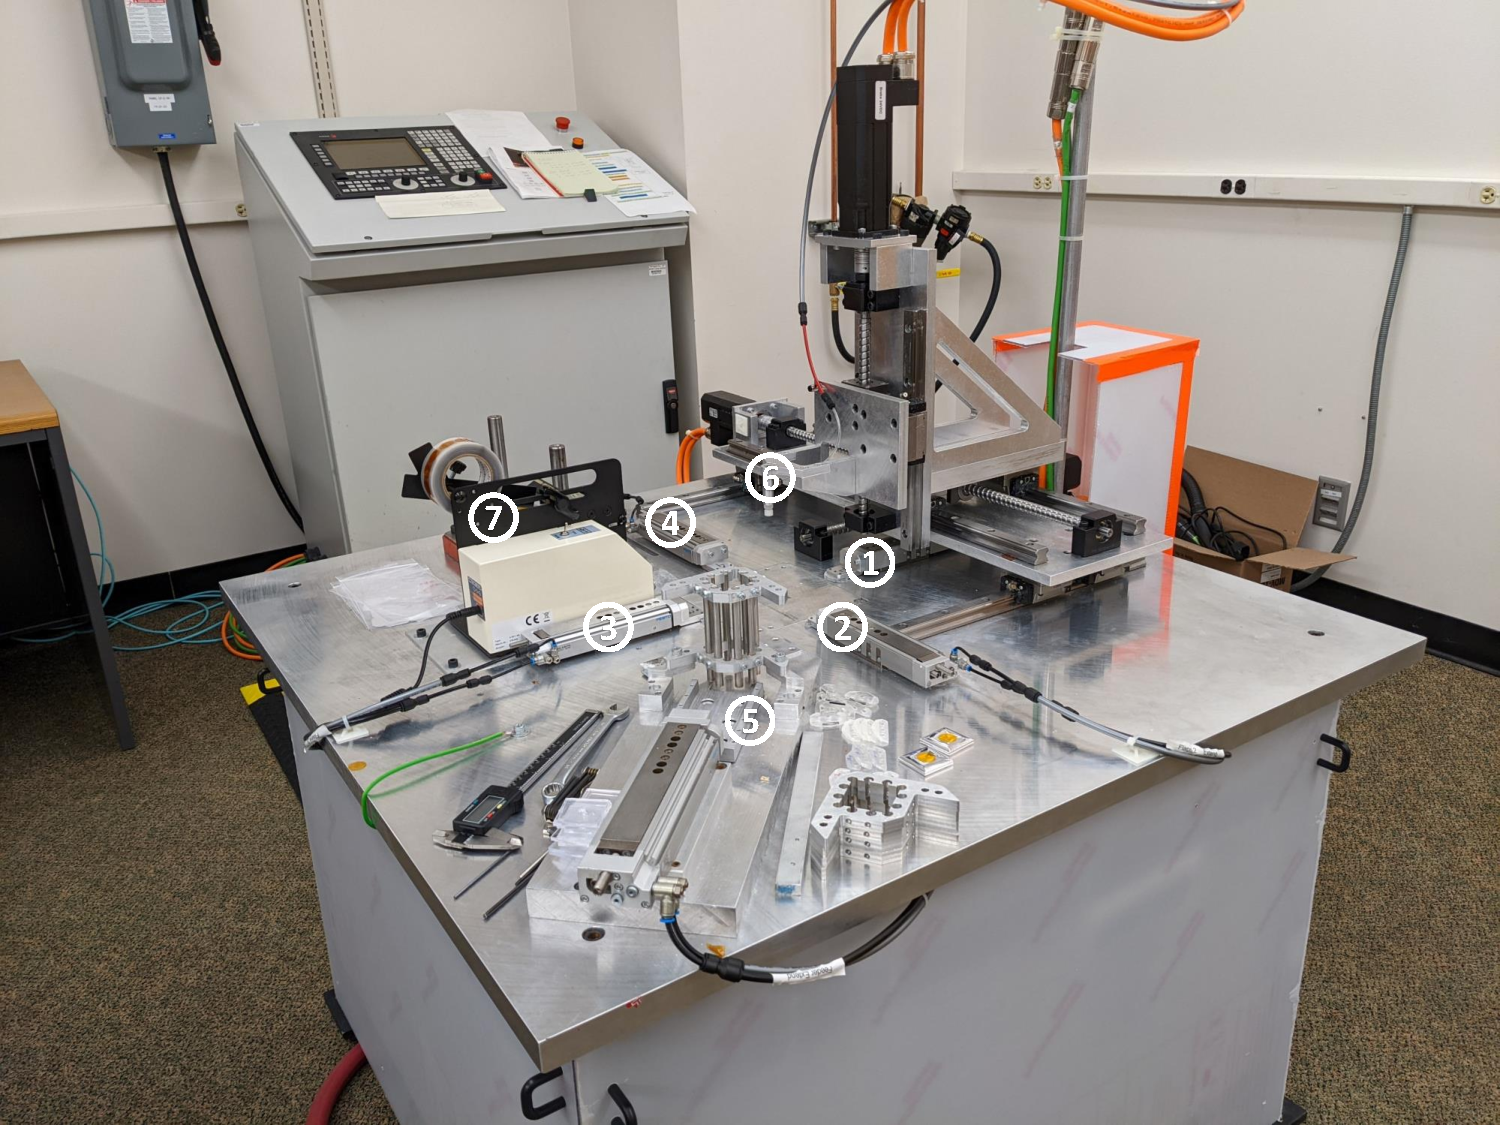
\includegraphics[width=\textwidth,page=1]{figures/wrapper_machine_pics.pdf}
  \caption[Automated scintillator tile wrapper overview]
  {Automated scintillator tile wrapper overview. Shown in picture with labels are,
    1--4: Actuator arms for folding the cut ESR flaps over the tiles,
    5: Tile magazine and dispenser assembly, 6: \textit{z}-axis (vertical up/down) end-effector
    with vacuum suction, 7: Kapton sticker dispenser.}%
  \label{fig:wrapper-overview-1}
\end{figure}

The machine is built to provide precise motion in \textit{xyz}-axes
and controlled by a computer numerical control (CNC) using G-code programming language.
One of the key components of the wrapper machine are actuators
which have arms that can extend and retract quickly with the
pressurized air. The wrapper uses both pressurized air and vacuum which
are controlled
by a solenoid switch using a
programmable logic controller running in G-code programs.

\begin{figure}[!ht]
  \centering
  \includegraphics[width=\textwidth,page=2]{figures/wrapper_machine_pics.pdf}
  \caption[Tile folding station and ESR magazine]
  {Tile folding station and ESR magazine. Shown in picture
    with labels 1: tile folding station, and 2: ESR magazine.}%
  \label{fig:wrapper-overview-2}
\end{figure}

The final wrapped tile as shown in Figure~\ref{fig:hgcal-scintillator-tile-wrapped}
is done by the machine in following steps:

\begin{itemize}
  \item \textbf{ESR Pickup, and Placement}: \textit{z}-axis (vertical up/down) end-effector
        picks up the cut \gls{ESR} using vacuum suction from the \gls{ESR} magazine,
        and then places it precisely over the tile pocket in the folding station.
        Placed \gls{ESR} over tile pocket is held into its place with
        the help of vacuum suction, which is built into the tile pocket
        seat.
  \item \textbf{Tile Dispenser, Pickup, and Placement}:
        Tiles will be stacked in the magazine at the tile dispenser
        location and an actuator arm will push out a tile
        completely and hold in place (right image in Figure~\ref{fig:wrapper-overview-3}) until the \textit{z}-axis end-effector
        makes contact and vacuum suction is turned on. Now,
        the actuator arm is retracted, and tile is
        picked up and placed over \gls{ESR} at the folding station.
  \item \textbf{ESR Flaps Folding}:
        After \gls{ESR} and tile have been placed, the tile pocket
        retracts with the help of actuator connected to it from the bottom.
        At this stage tile is inside pocket and flush with top of the table.
        \gls{ESR} flaps are out and vertical.
        Now the four actuator arms as shown in Figure~\ref{fig:wrapper-overview-4}
        extend and close \gls{ESR} flaps.
  \item \textbf{Sticker Application}:
        The folding actuator arms stay in place until sticker is
        applied using \textit{z}-axis end-effector which
        picks up the sticker from sticker dispenser (left image Figure~\ref{fig:wrapper-overview-3}) and applies it on
        the center of the tile where all flap corners meet.
  \item \textbf{Wrapped Tile}:
        Final step in wrapping is retracting the folding actuator arms,
        pushing out the tile and turning of the vacuum suction of the tile pocket.
        Now \textit{z}-axis end-effector picks up the wrapped tile and
        drops into the collection basket.
        Wrapped tile in Figure~\ref{fig:hgcal-scintillator-tile-wrapped}
        is wrapped automatically with this procedure.
\end{itemize}

\begin{figure}[!ht]
  \centering
  \includegraphics[width=0.49\textwidth,page=3]{figures/wrapper_machine_pics.pdf}
  \includegraphics[width=0.49\textwidth,page=4]{figures/wrapper_machine_pics.pdf}
  \caption[Sticker and tile dispenser.]
  {Sticker and tile dispenser, Left: Sticker dispenser
    with kapton tape roll. Right: Tile dispenser with tile magazine.}%
  \label{fig:wrapper-overview-3}
\end{figure}

\begin{figure}[!ht]
  \centering
  \includegraphics[width=0.49\textwidth,page=6]{figures/wrapper_machine_pics.pdf}
  \includegraphics[width=0.49\textwidth,page=7]{figures/wrapper_machine_pics.pdf}
  \caption[Tile folding station]
  {Tile folding station. Left: Flushed tile pocket at the center
    and retracted actuator arms. Right: After all the
    arms are extended during wrapping.}%
  \label{fig:wrapper-overview-4}
\end{figure}

\clearpage
\section{
  Signal-to-Noise Ratio
 }

As discussed earlier in the Section~\ref{ch_hgcal:technical-design},
for the \gls{HGCAL} to retain its performance till the end-of-life it needs
good \gls{SNR}, which is defined as \gls{SNR} \( > 3\). In this section we
will discuss formulation and inputs to the \gls{SNR} calculation, and
the results of optimal configuration by minimizing cost and
retaining good \gls{SNR}.

\subsection{
  Formulation
}

Signal-to-Noise formulation is based detecting \glsfirstplural{MIP}.
For the scintillator tile coupled directly with SiPM is formulated as~\cite{cms-dn-17-001}:

\begin{equation}
  \frac{S}{N} =
  \frac{
  (\texttt{MIP}_\texttt{response})
  \sqrt{\frac{A_{t,\texttt{ref}}}{A_{t}}}
  \left(\frac{A_{s}}{A_{s,\texttt{ref}}}\right)
  (\texttt{Radiation Loss})
  }
  {
  (\texttt{SiPM}_\texttt{noise,base})
  \sqrt{\frac{A_{s}}{A_{s,\texttt{base}}}}
  \sqrt{1.88^{\frac{T_{s}-T_{s,\texttt{base}}}{10^{\circ} \text{ C}}}}
  \sqrt{\frac{f}{f_{\texttt{base}}}}
  }
\end{equation}

where,

\begin{itemize}
  \item \( \texttt{MIP}_\texttt{response} \): measured in \gls{PE} is the
        response of the scintillator tile light yield with a scale factor to account for \gls{SiPM} device
        \gls{PDE} difference used during testbeam measurement and
        \gls{SiPM} expected to be used.
  \item \( A_t \): is the area of the tile for which the \gls{SNR} is being
        evaluated and subscript \( \texttt{ref} \) means the area of tile
        used in the testbeam \gls{MIP} measurement.
  \item \( A_s \): the active area of the
        \gls{SiPM} device coupled to scintillator tile.
  \item \( \texttt{Radiation Loss} \): is the loss in light output
        of the scintillator
        due to the radiation dose received, it is expressed as:
        \begin{gather}
          e^{-R/D_{c}} \\
          D_c = (6.0 \text{ Mrad})
          {\left( \frac{R}{1 \xspace\text{ krad/hr}} \right)}^{0.35}
        \end{gather}
        where \( R \) is the dose rate in \( \text{krad/hr} \), and \( D_c \) is the
        dose constant, and both are obtained from \textsc{FLUKA} simulations.
  \item \( \texttt{SiPM}_\texttt{noise,base} \):
        is the \gls{RMS} value in \gls{PE} of
        intrinsic noise of \glspl{SiPM} from thermal excitations
        (also called \gls{DCR}),
        irradiation of silicon also increases this noise.
  \item \( T_{s,\texttt{base}}\): temperature of the \glspl{SiPM} during
        \gls{DCR} measurement.
  \item \( A_{s,\texttt{base}}\): active area of the \glspl{SiPM} used during
        \gls{DCR} measurement.
  \item \( f_{\texttt{base}}\): fluence used to the irradiate \glspl{SiPM} for  \gls{DCR} measurement.
  \item \( T_s \): is the temperature of the \gls{HGCAL} hence the \gls{SiPM}
        at which it will be operated, which is \( -30^\circ \text{ C} \).
  \item \( f \): is the fluence the \gls{SiPM} depending on its location will receive over its
        lifetime of operation in \gls{HGCAL}.
\end{itemize}

\subsection{
  Testbeam and SiPM Noise Inputs
}

\gls{CMS} \gls{HGCAL} collaboration conducted testbeam measurement in January 2020 on both cast and injection
molded scintillator tiles wrapped in \gls{ESR} with \gls{SiPM}
using \gls{FNAL} 120 \GeV{} testbeam facility. The scintillator tiles
used in testbeam were of dimensions \( 30 \times 30 \mm{}^{2} \) square tiles,
and \gls{SiPM} device used was Hamamatsu S13360--1350CS (\( 1.3 \times 1.3 \mm{}^{2} \))
~\cite{mppc-13360,testbeam-fnal-2020}.

The scintillator tiles response measured from testbeam are 35 \gls{PE} for cast scintillator tiles,
and 25 \gls{PE} for injection molded with \gls{SiPM} operated at
voltage of 54.26 V, which is \gls{OV} of 2.5V (I-V method) (equivalent
to 3.0V when measured with gain method).
Currently \gls{SiPM} device class expected to used in \gls{HGCAL}
is Hamamatsu S14160 with 15\micron{} pixel size (dubbed as HDR15)
and \(2, 4, 9 \mm{}^{2} \) in
area operated at \gls{OV} of 2V (I-V method),
using ratio of \glspl{PDE} of these devices
we can calculate PDE scale factor as,

\begin{equation}
  = \frac{\text{PDE of S14160 at } V_O = 2V}
  {\text{PDE of S13360 at } V_O = 3V}
  = \frac{34.9}{40}
  = 0.8725
\end{equation}

this gives, \( \texttt{MIP}^{*} \) value to be 30.5 \gls{PE} for cast
and 21.8 \gls{PE} for injection molded scintillator tiles.

\gls{DCR} measurement for HDR15 (\( 2 \mm{}^2 \)) \glspl{SiPM}
irradiated to \( 5 \times {10}^{13} \text{ n}/\cm{}^2 \)
operated at \gls{OV} = 2V (I-V method) and at temperature \( -30^{\circ} \text{ C}\)
is equivalent to \gls{RMS} value of 19 \gls{PE} with 15 \nanoseconds{} integration time
period~\cite{dark-current-measurement}.

Using the testbeam measurement of scintillator tile response and irradiated \gls{SiPM}
\gls{DCR} measurements end-of-life scenario estimation of
detector performance was done for combinations
of scintillator types and HDR15 \glspl{SiPM} areas.

\subsection{
  Scenarios
}

Five combinations of scintillator material and \gls{SiPM} active area
were considered and for each combination the detector
performance was evaluated. If there are
multiple options passing \gls{SNR} \(> 3\) requirement for the same tileboard,
the option with the higher preference is selected. Two different scenarios were
considered with preference order as:

\begin{itemize}
  \item \textbf{Scene A}:
        \begin{enumerate}
          \item Injection Molded Scintillator Tiles and SiPM of active area \( 2\mm{}^2 \).
          \item Injection Molded Scintillator Tiles and SiPM of active area \( 4\mm{}^2 \).
          \item Cast Scintillator Tiles and SiPM of active area \( 2\mm{}^2 \).
          \item Cast Scintillator Tiles and SiPM of active area \( 4\mm{}^2 \).
          \item Cast Scintillator Tiles and SiPM of active area \( 9\mm{}^2 \).
        \end{enumerate}
  \item \textbf{Scene B}:
        \begin{enumerate}
          \item Injection Molded Scintillator Tiles and SiPM of active area \( 2\mm{}^2 \).
          \item Cast Scintillator Tiles and SiPM of active area \( 2\mm{}^2 \).
          \item Injection Molded Scintillator Tiles and SiPM of active area \( 4\mm{}^2 \).
          \item Cast Scintillator Tiles and SiPM of active area \( 4\mm{}^2 \).
          \item Cast Scintillator Tiles and SiPM of active area \( 9\mm{}^2 \).
        \end{enumerate}
\end{itemize}

\gls{SNR} of each combination after 300 \fbinv{} when used alone is shown in
Figure~\ref{fig:hgcal-scint-everywhere}.
Injection molded scintillator can be used in the deeper layers,
and the cast scintillator with \(9 \mm{}^{2}\) \gls{SiPM} will be required
for starting layers.

\begin{figure}
  \centering
  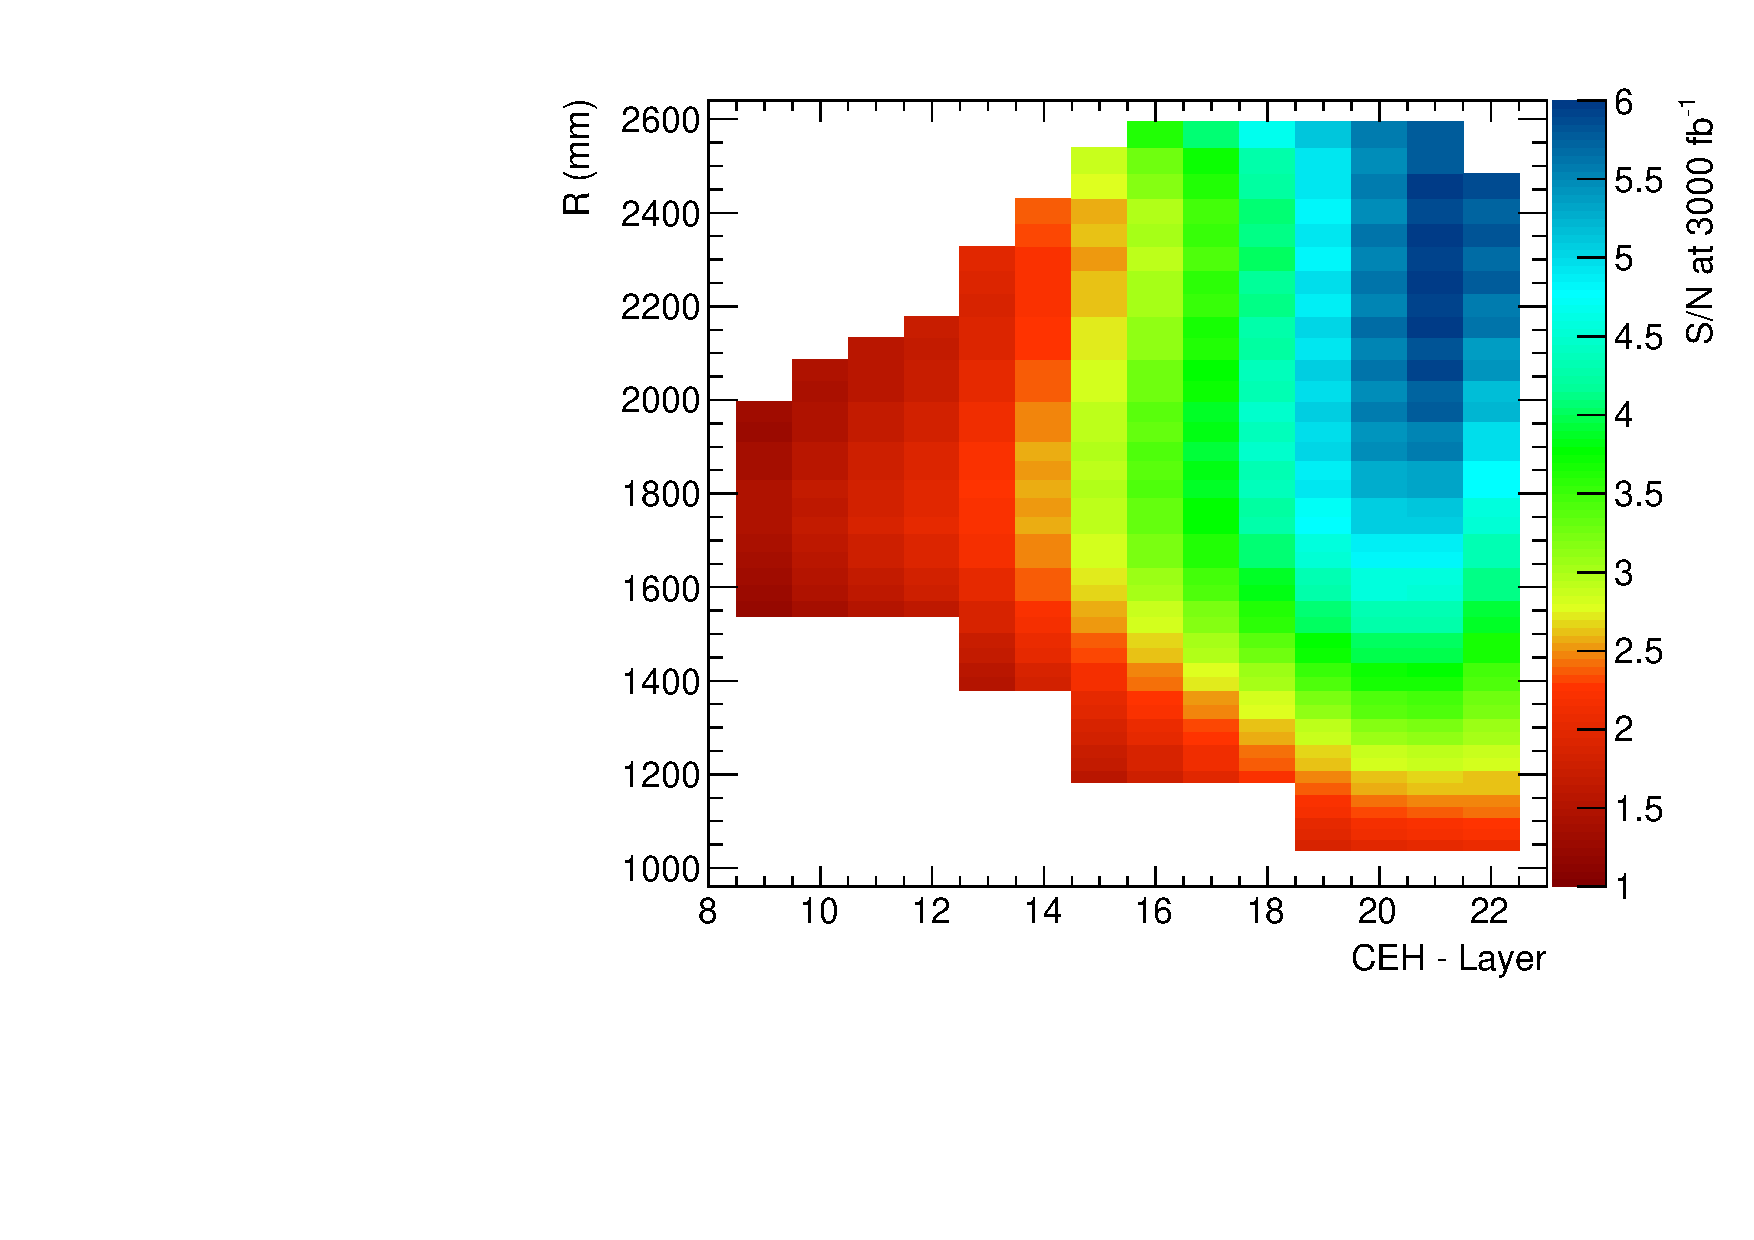
\includegraphics[width=0.45\textwidth]{figures/hgcal/plot_zr/mold_mip_25_pdeC_34.9_40_sipmA_2.0_rad_4_sipmN_52_sipmAC_default_tileAC_default_S_N.pdf}\\
  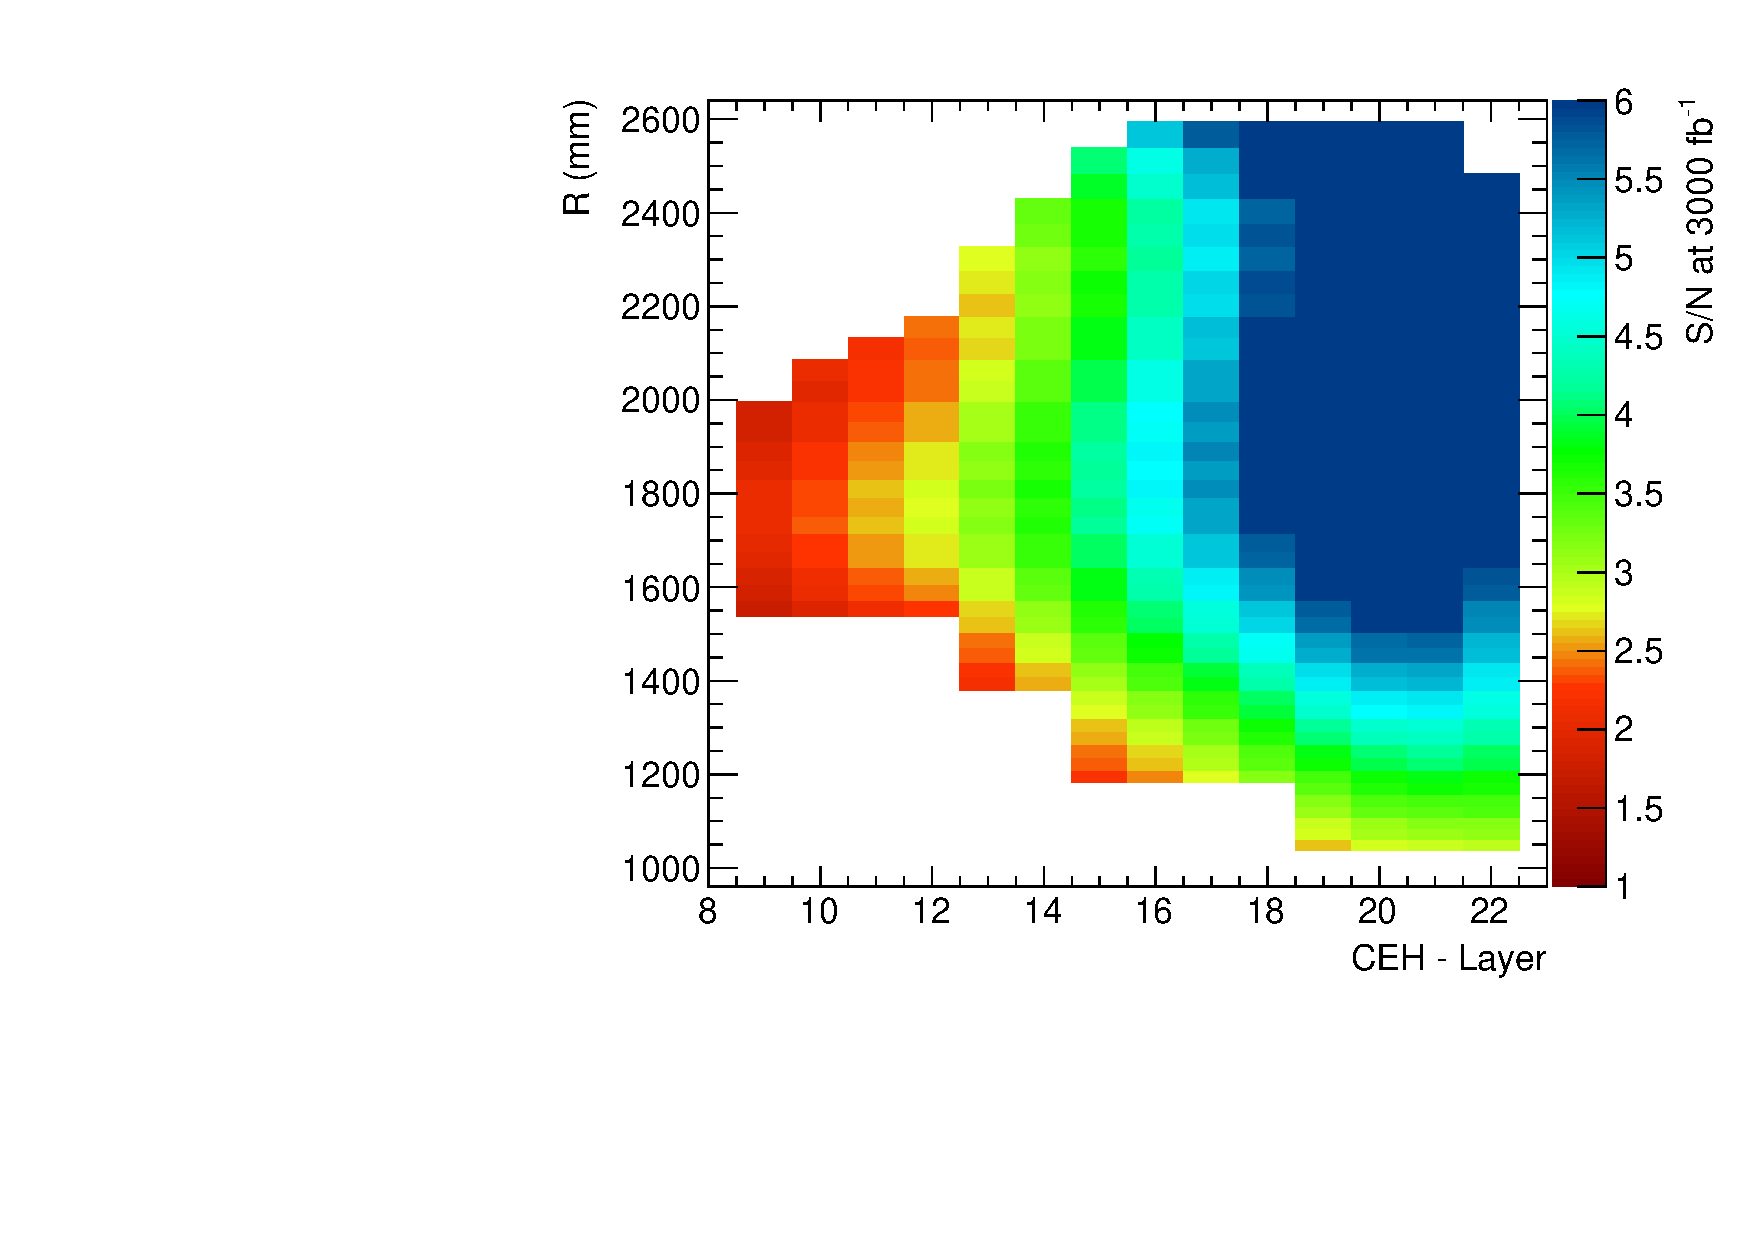
\includegraphics[width=0.45\textwidth]{figures/hgcal/plot_zr/mold_mip_25_pdeC_34.9_40_sipmA_4.0_rad_4_sipmN_52_sipmAC_default_tileAC_default_S_N.pdf}
  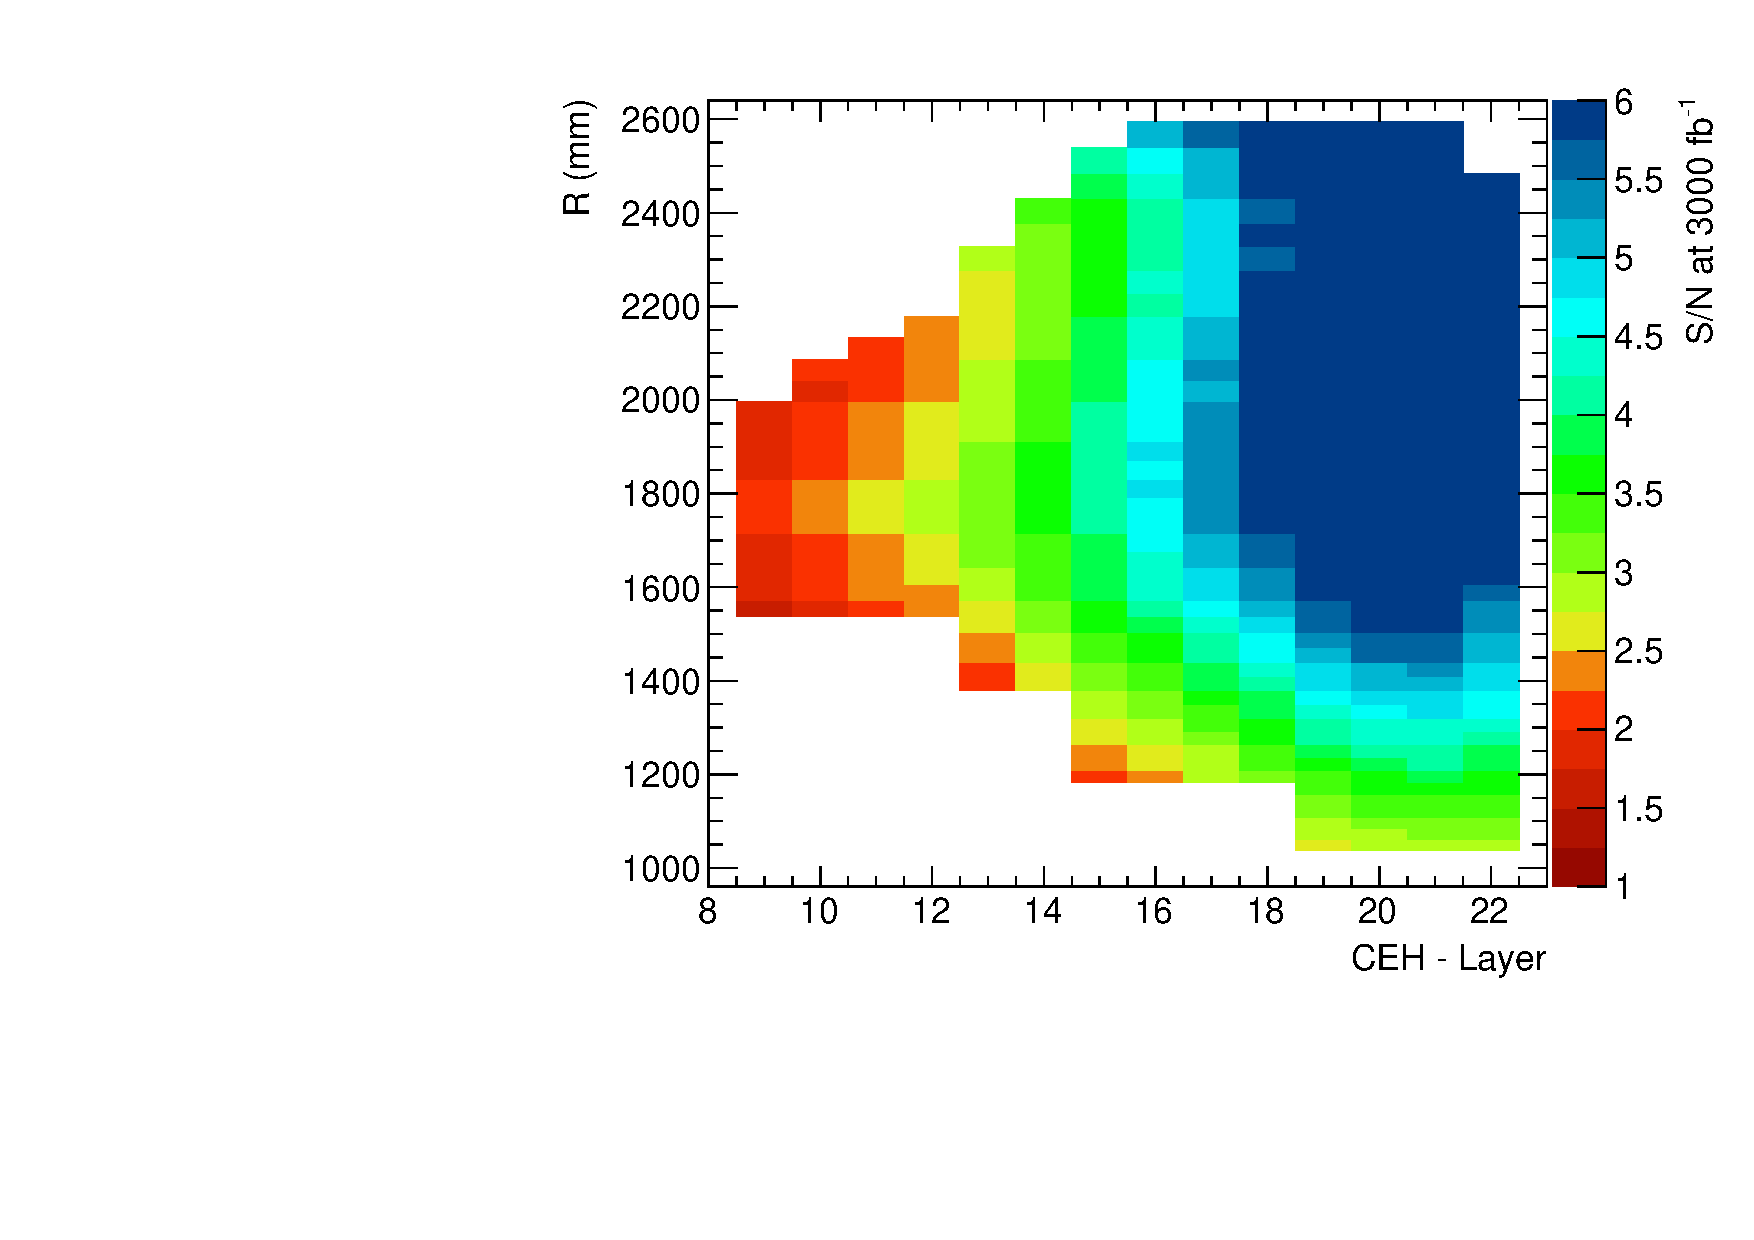
\includegraphics[width=0.45\textwidth]{figures/hgcal/plot_zr/cast_mip_35_pdeC_34.9_40_sipmA_2.0_rad_4_sipmN_52_sipmAC_default_tileAC_default_S_N.pdf}\\
  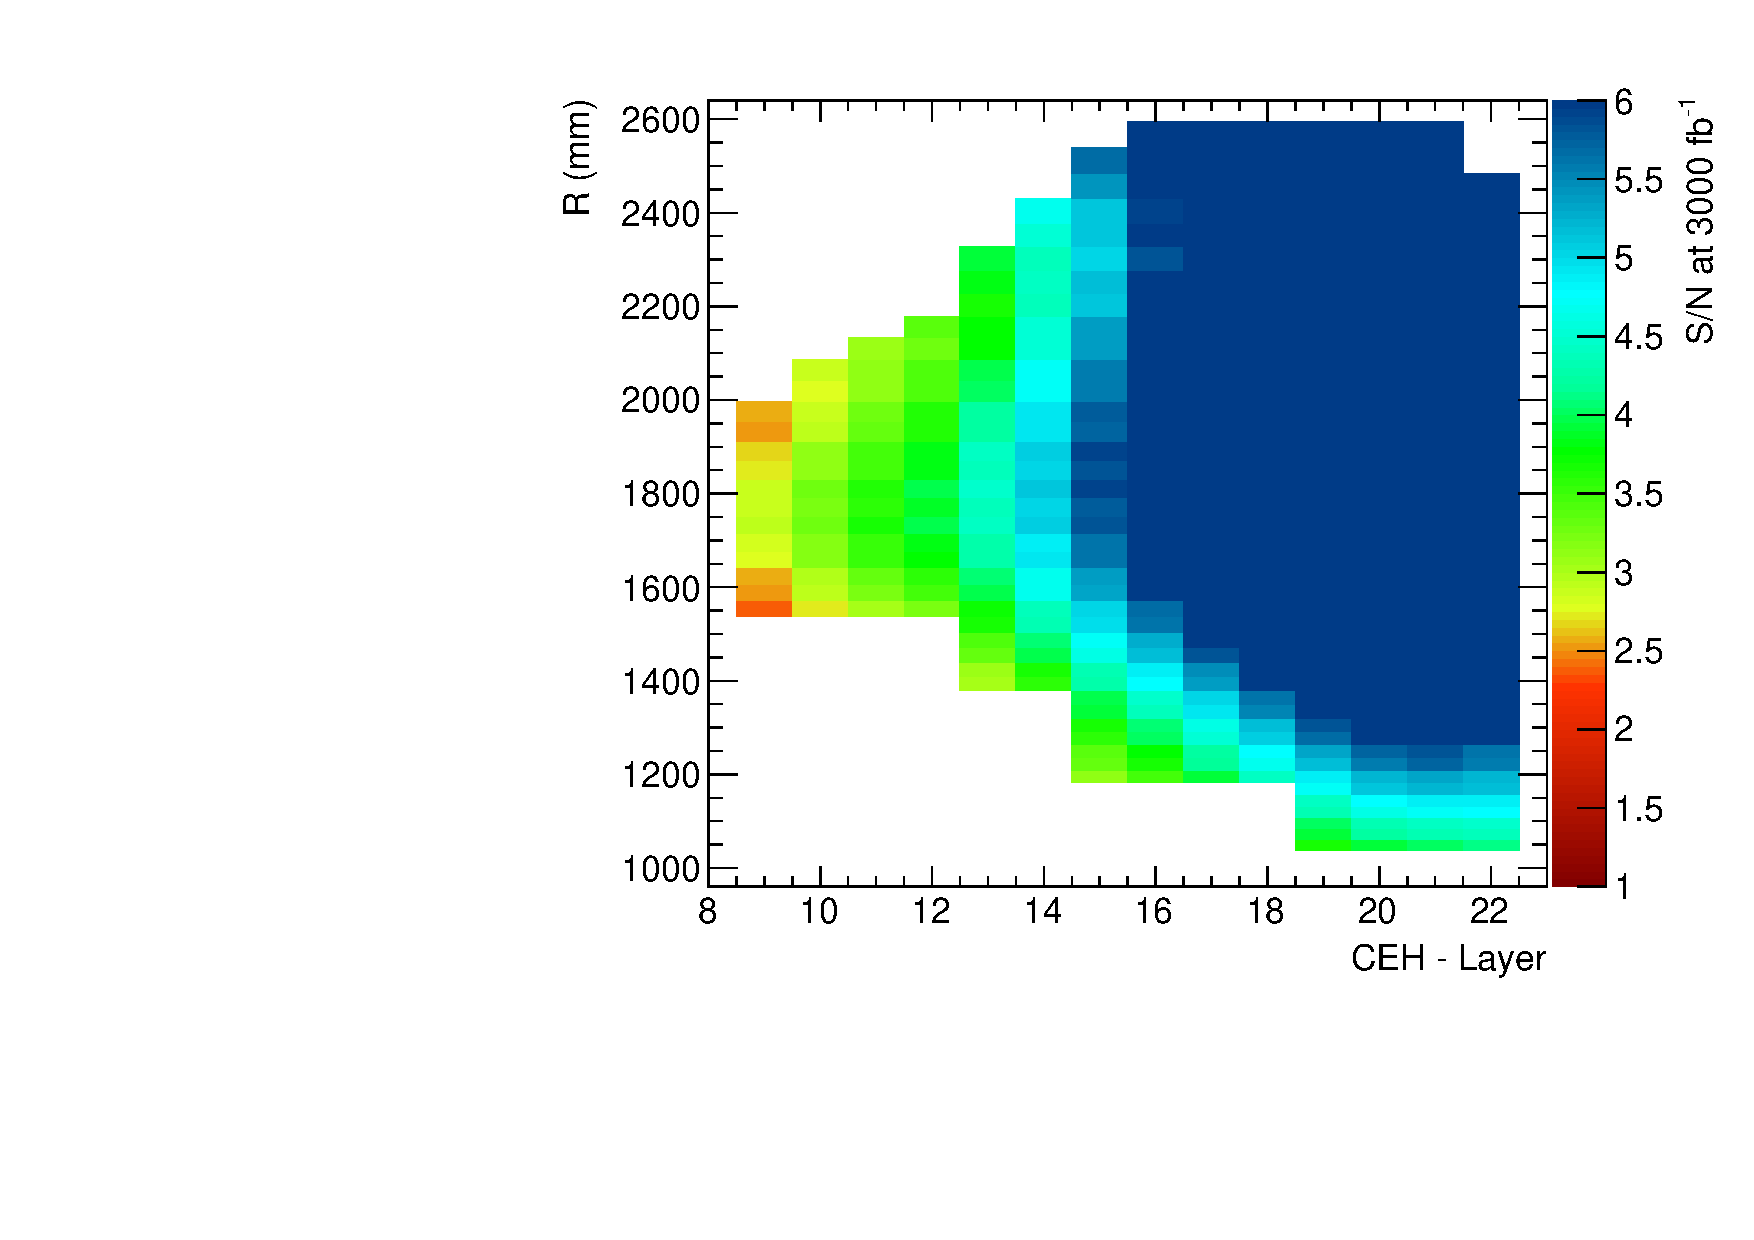
\includegraphics[width=0.45\textwidth]{figures/hgcal/plot_zr/cast_mip_35_pdeC_34.9_40_sipmA_4.0_rad_4_sipmN_52_sipmAC_default_tileAC_default_S_N.pdf}
  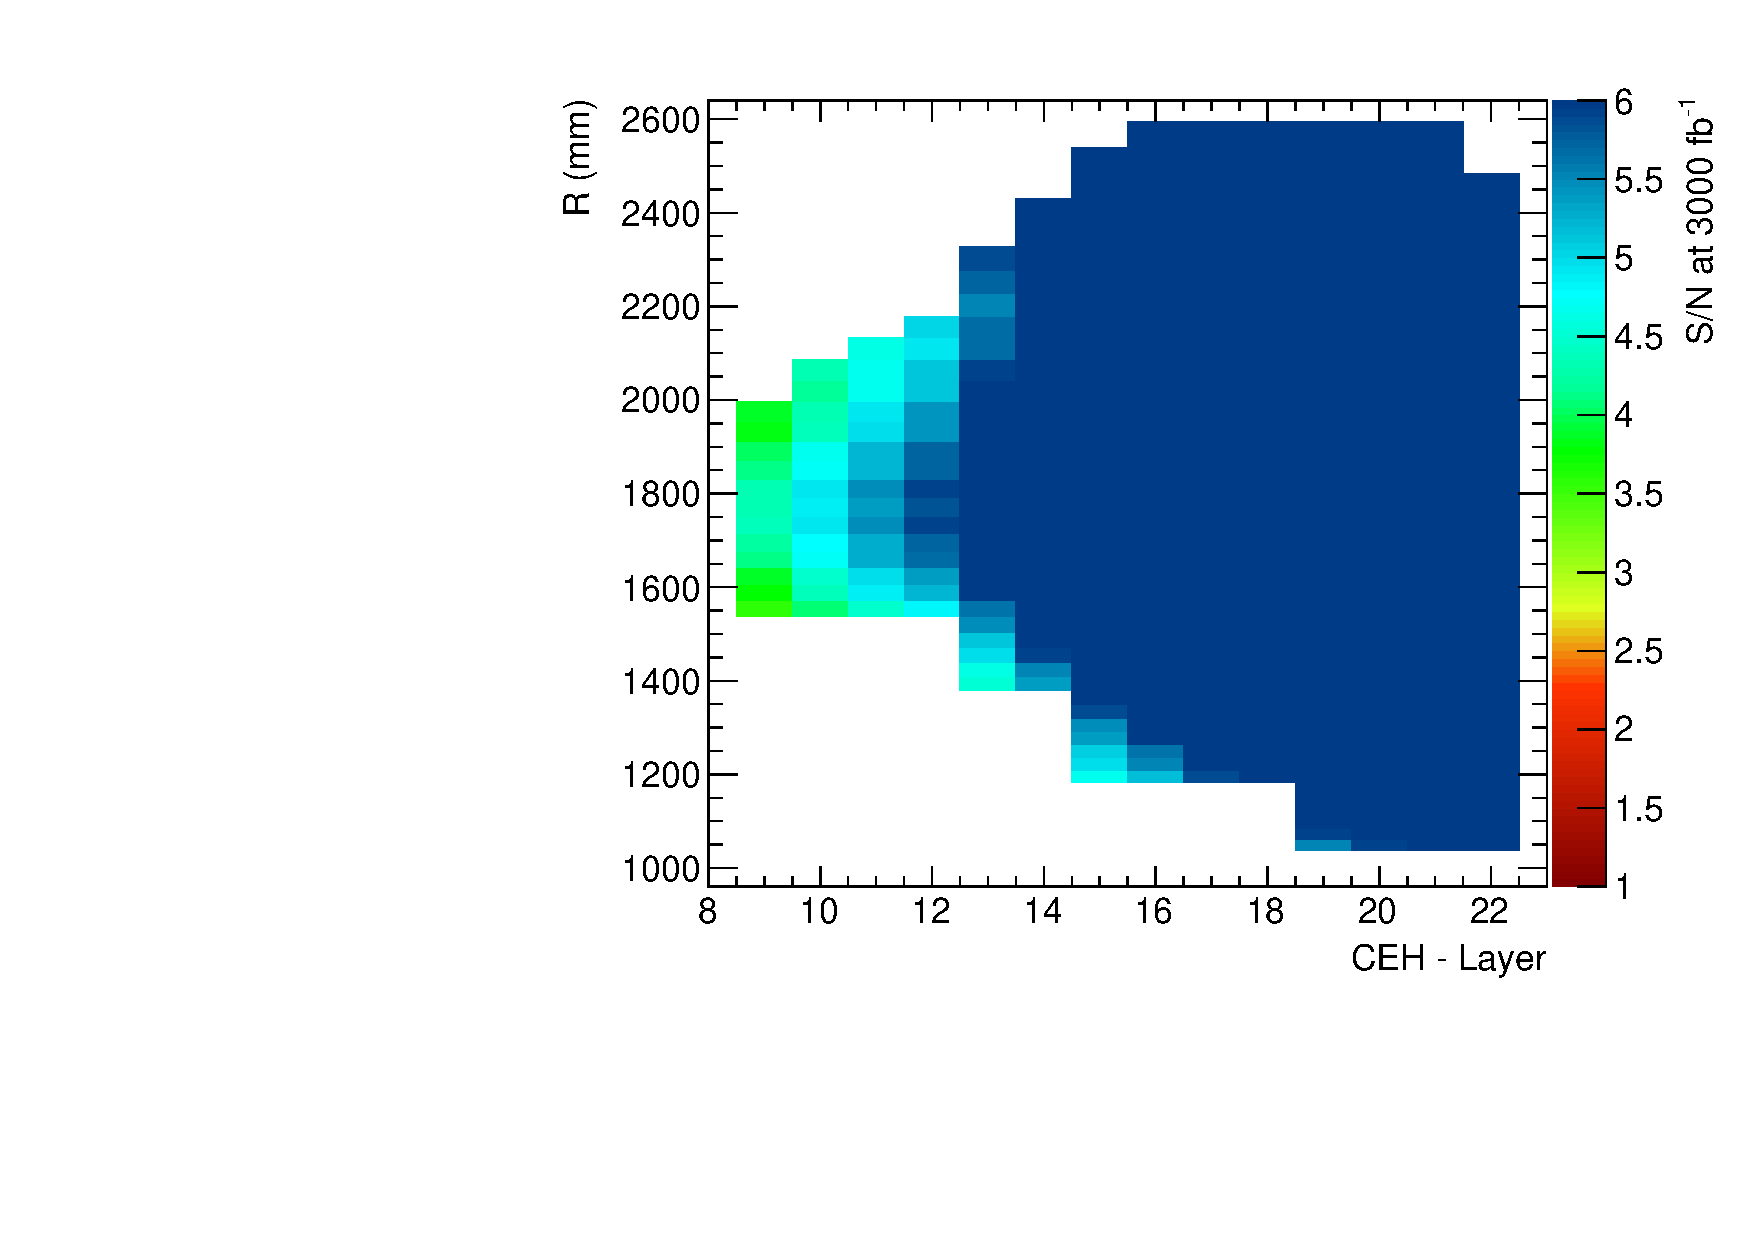
\includegraphics[width=0.45\textwidth]{figures/hgcal/plot_zr/cast_mip_35_pdeC_34.9_40_sipmA_9.0_rad_4_sipmN_52_sipmAC_default_tileAC_default_S_N.pdf}
  \caption[Scintillator performance with various active area size
    of \gls{SiPM}]{Scintillator performance with various active area size
    of \gls{SiPM}. Top row from Left to Right: Injection Molded
    Scintillator with \gls{SiPM} \( 2 \) and \( 4\mm{}^2 \) active area device.
    Bottom row from Left to Right: Cast Scintillator with
    \gls{SiPM} \( 2,4 \) and \( 9\mm{}^2 \) active area device.}%
  \label{fig:hgcal-scint-everywhere}
\end{figure}

\subsection{
  Results and Conclusion
}

Since for assembly of scintillator tiles on tileboard, it is preferred
to have single type of scintillator with \gls{SiPM} combination.
For this reason, each scene is evaluated in the preference order
and tileboard is assigned a combination only
if all the rings in it are able to satisfy \gls{SNR} \( > 3\).
Figure~\ref{fig:hgcal-scenes-fnal-jan20} shows final
results of how both scenes fill tileboards in \gls{CE-H}.

\begin{figure}[!ht]
  \centering
  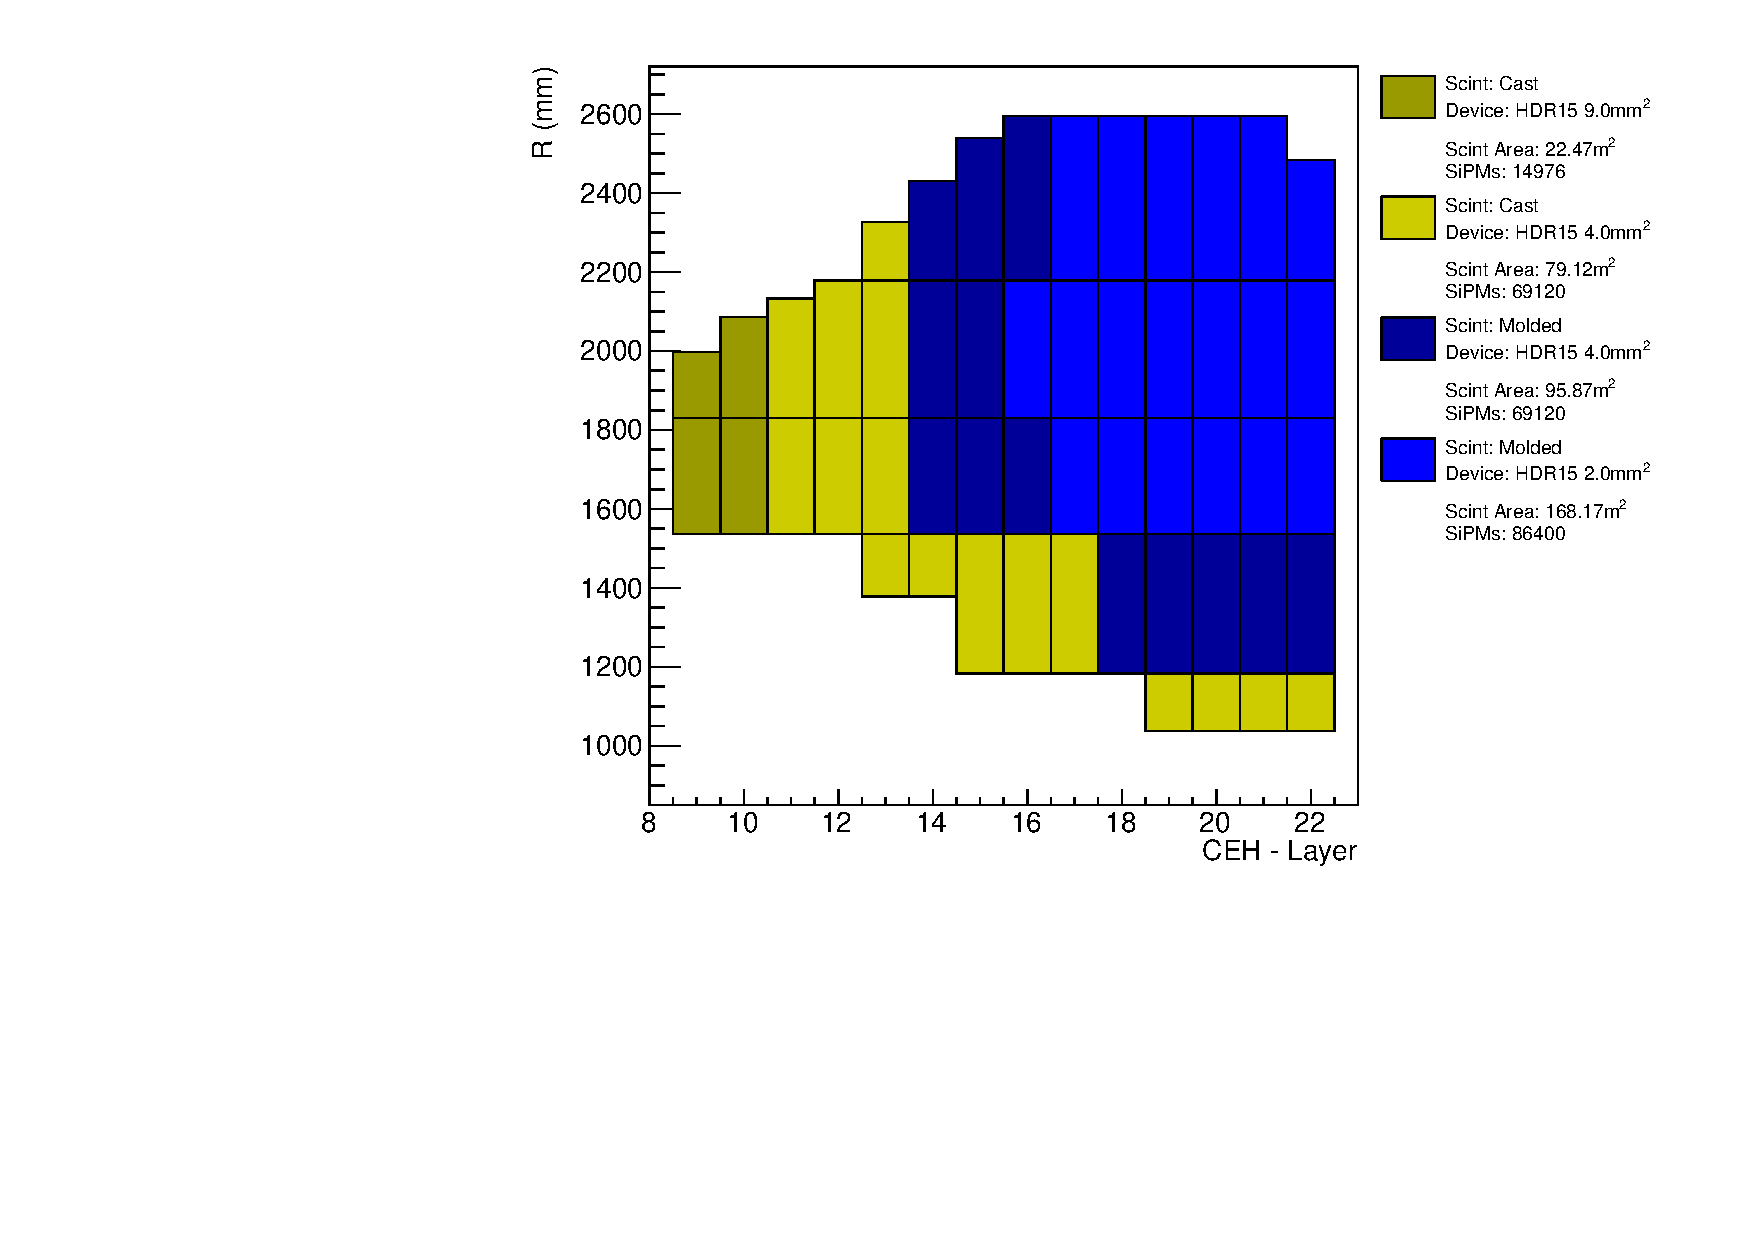
\includegraphics[trim={400 370 20 10},clip,width=0.24\textwidth]{figures/hgcal/plot_scenes/sceneA_jan20_fix_vto2p0_with9mm2.pdf}
  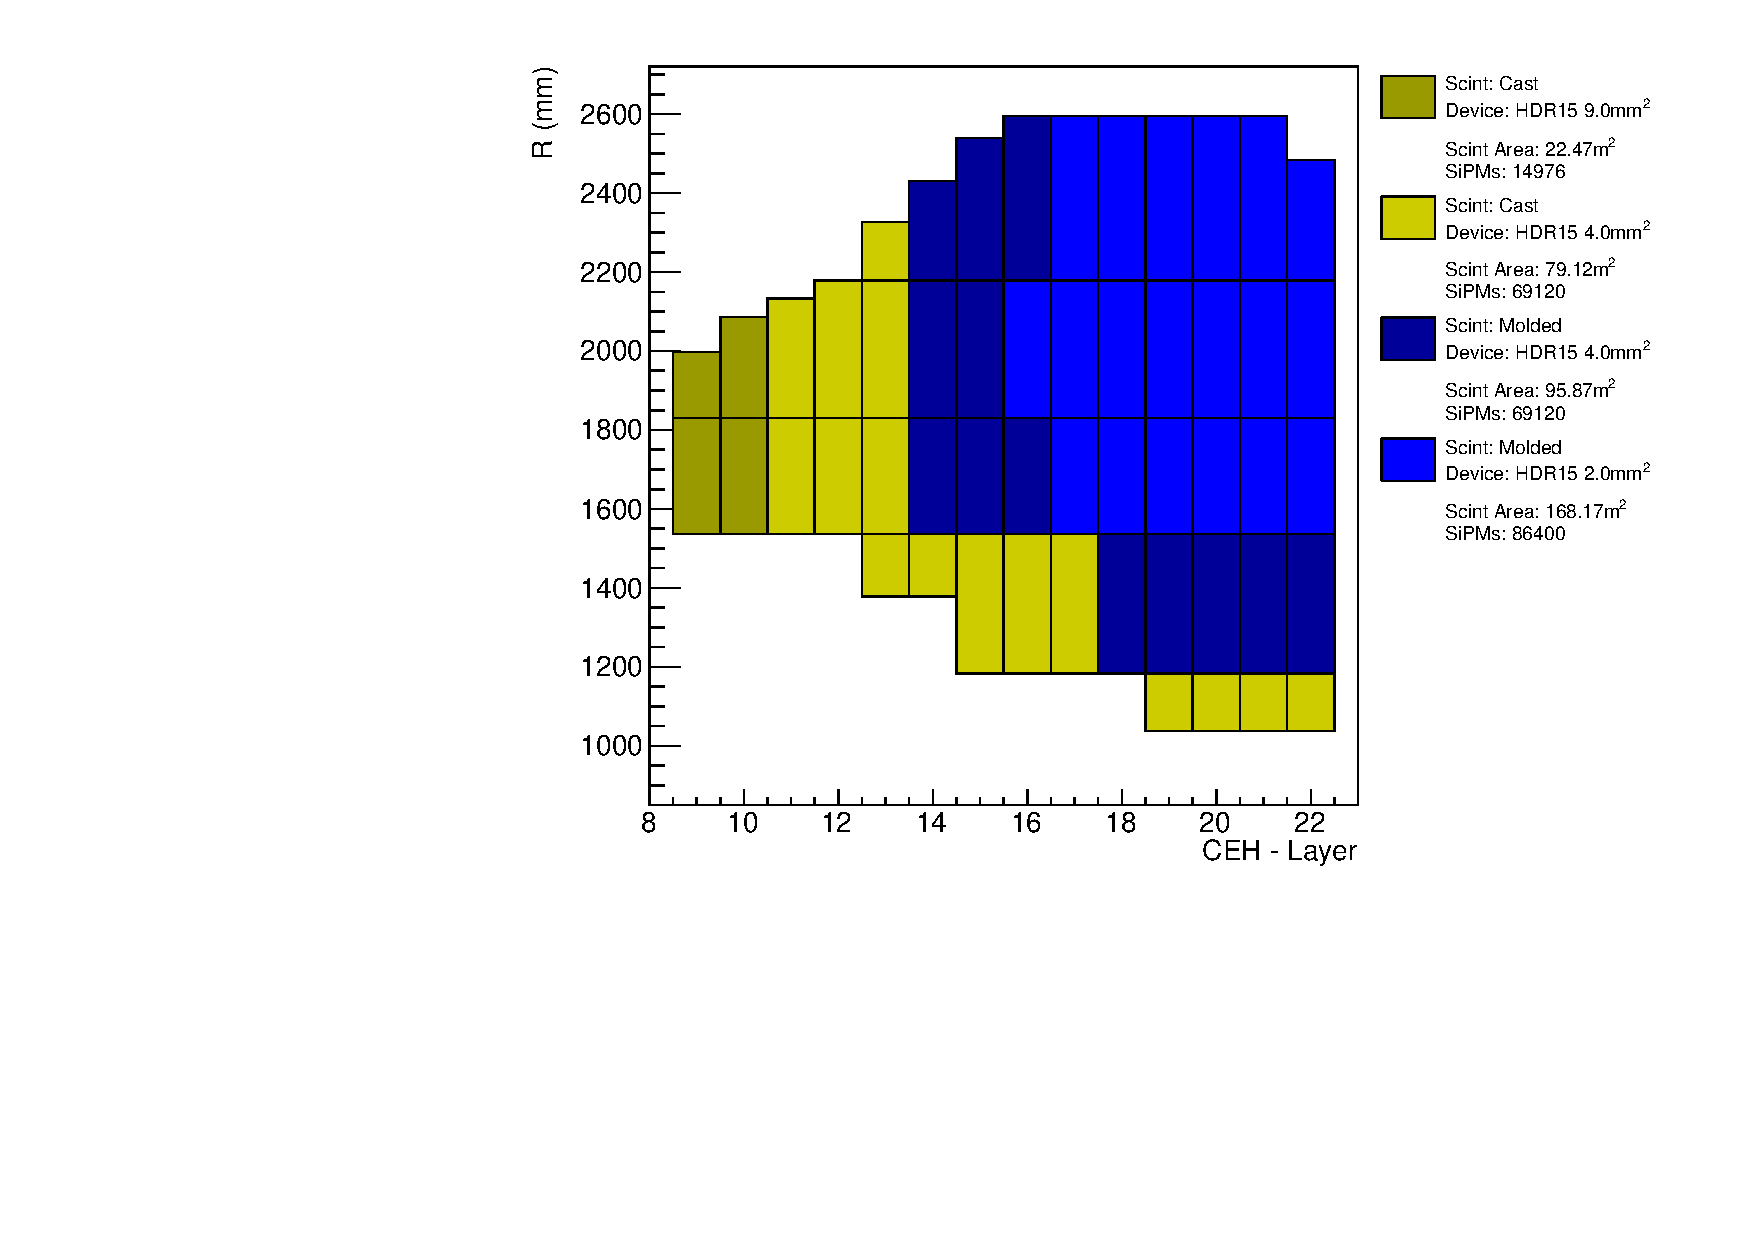
\includegraphics[trim={400 310 20 70},clip,width=0.24\textwidth]{figures/hgcal/plot_scenes/sceneA_jan20_fix_vto2p0_with9mm2.pdf}
  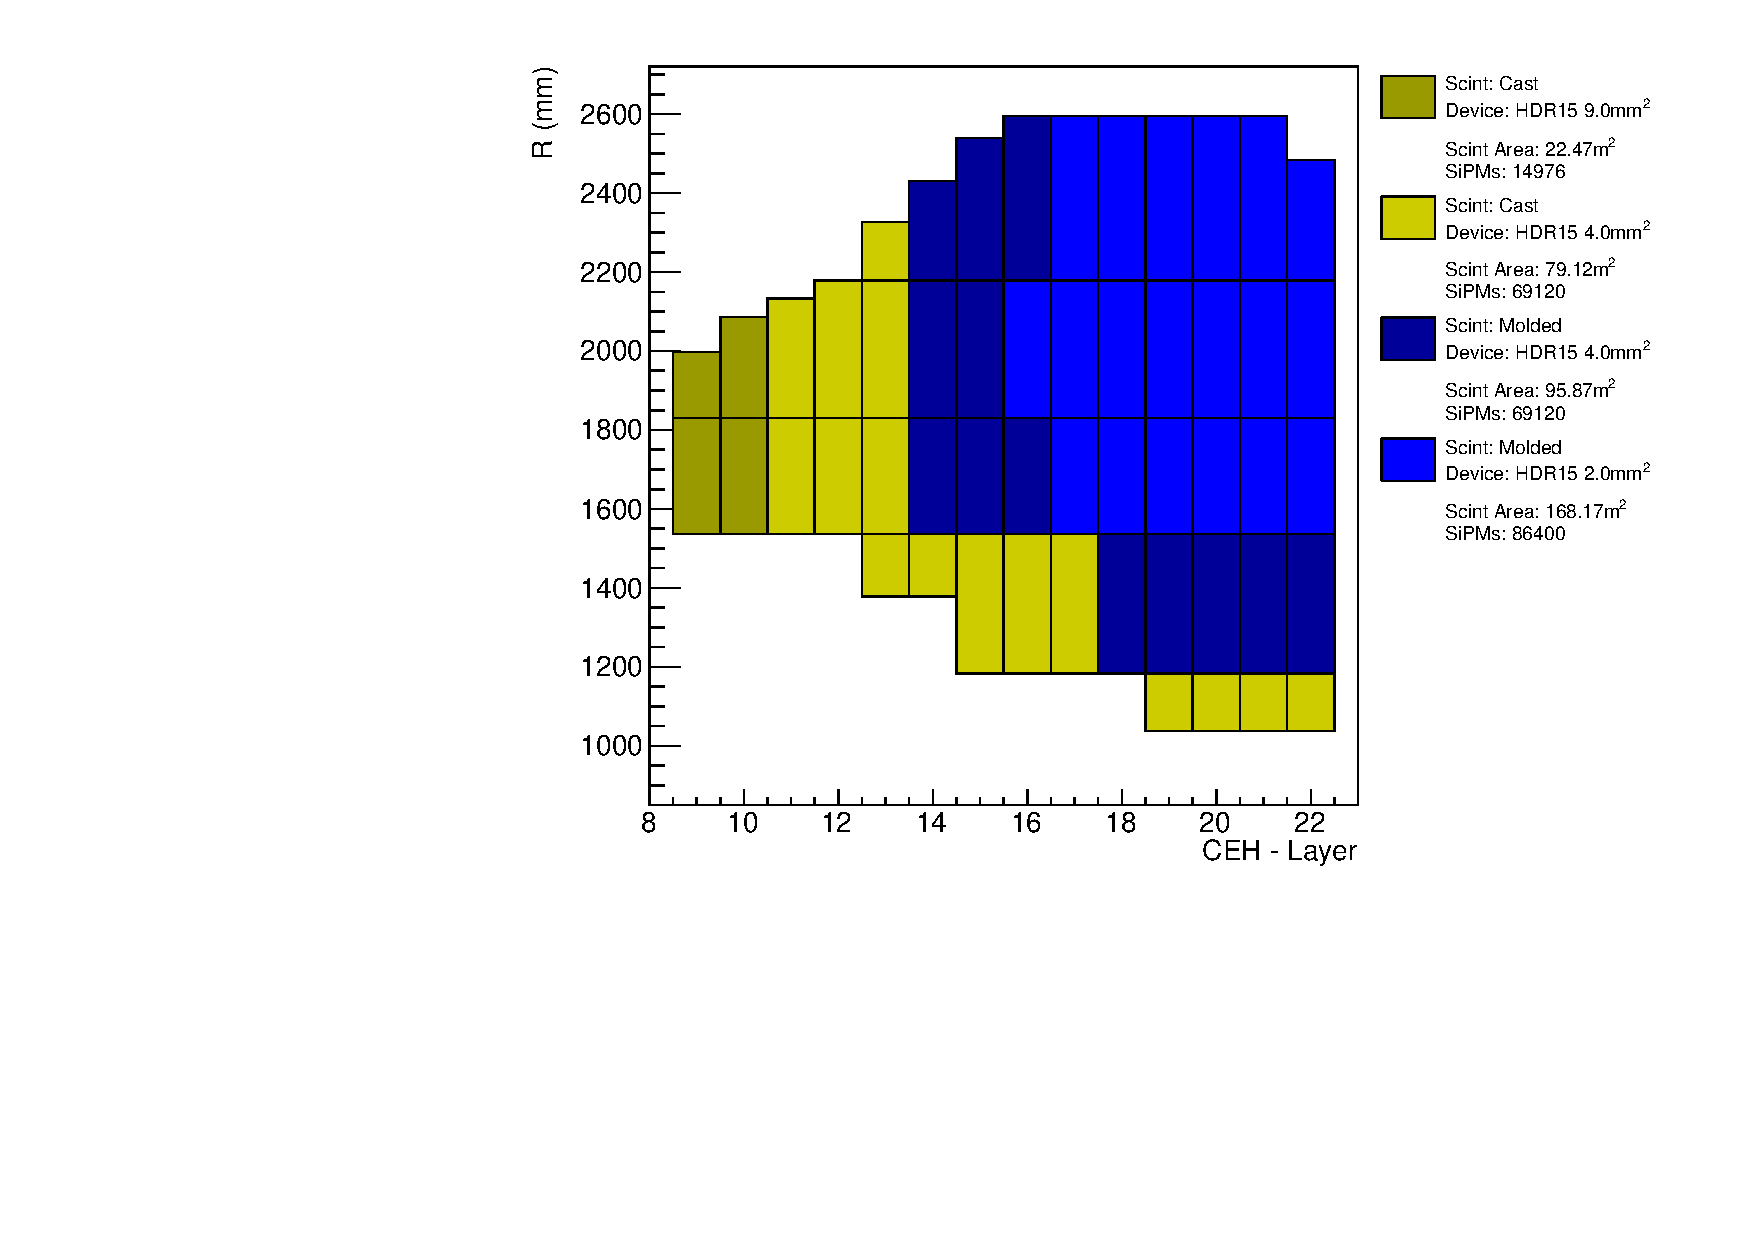
\includegraphics[trim={400 250 20 130},clip,width=0.24\textwidth]{figures/hgcal/plot_scenes/sceneA_jan20_fix_vto2p0_with9mm2.pdf}
  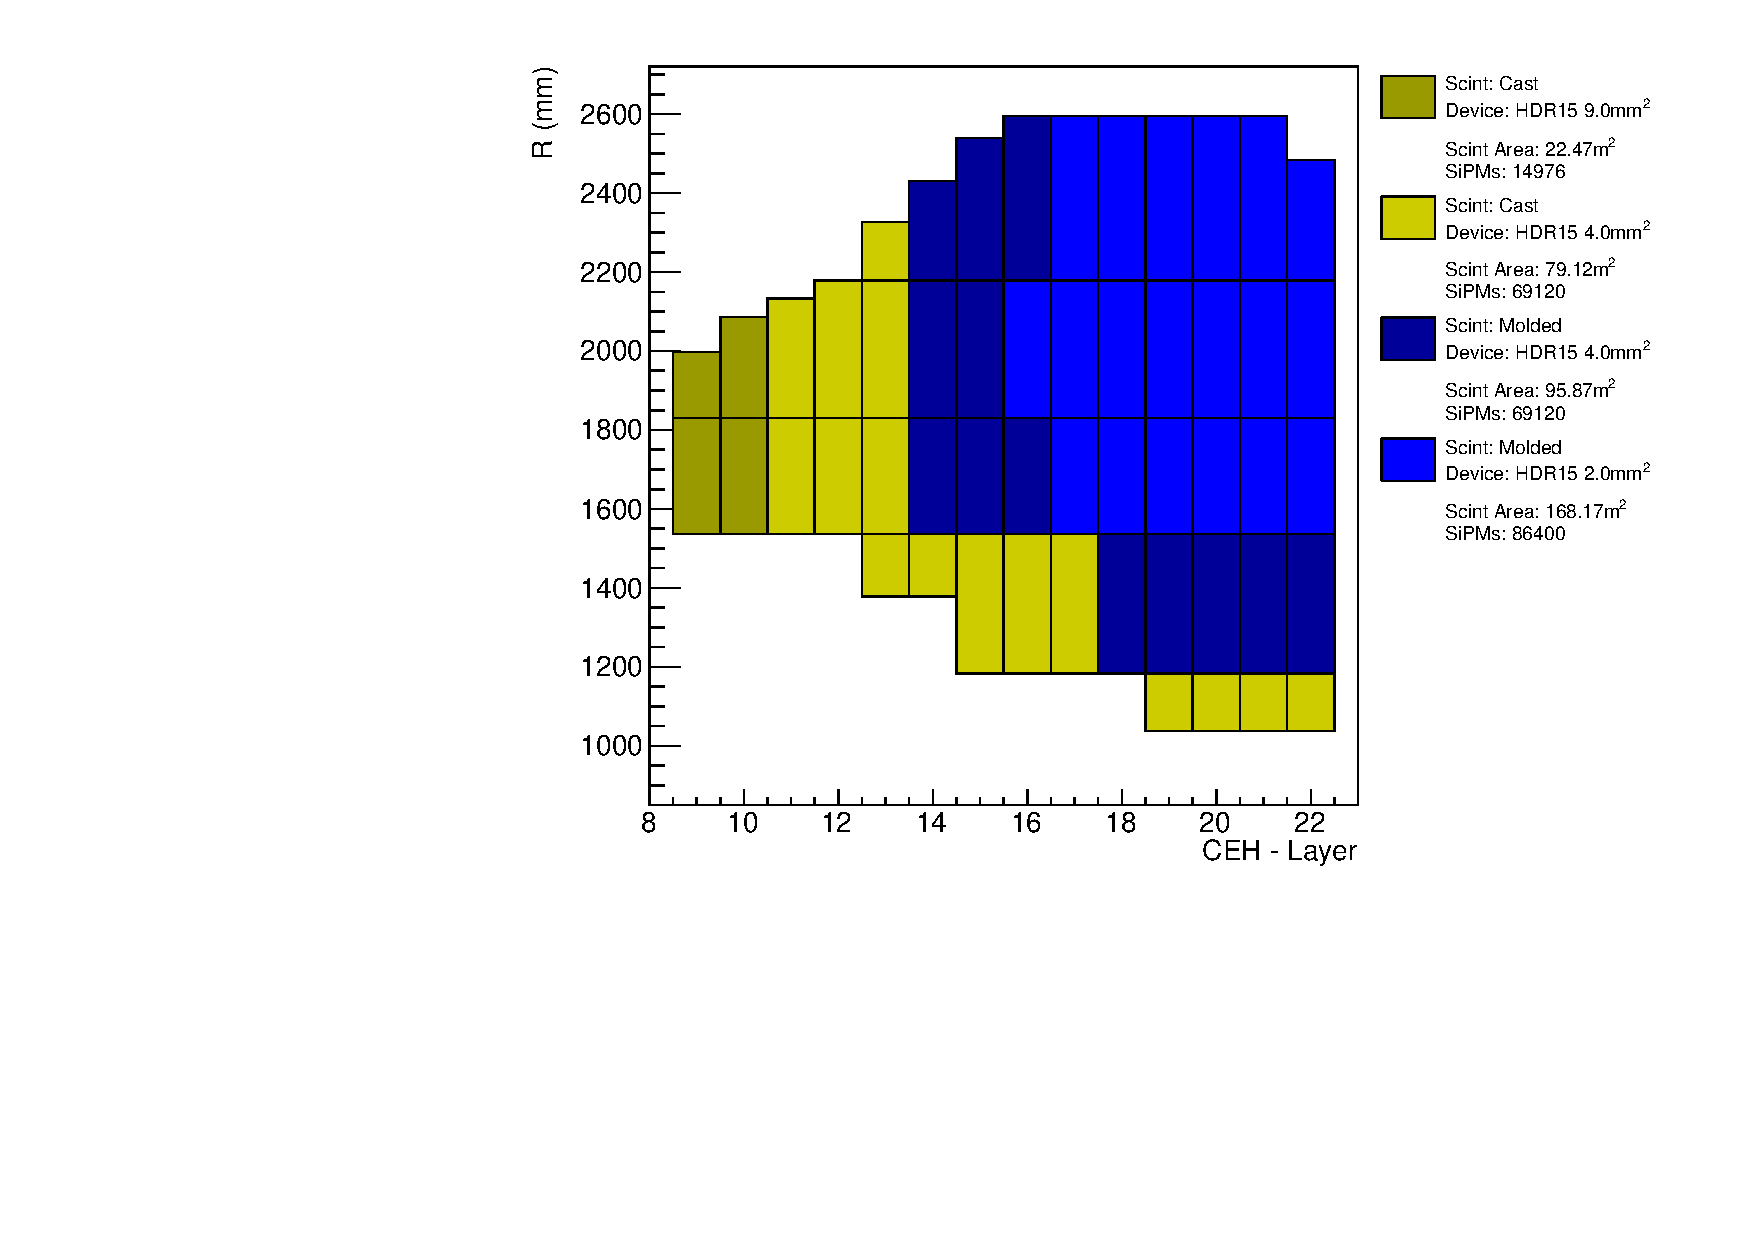
\includegraphics[trim={400 190 20 190},clip,width=0.24\textwidth]{figures/hgcal/plot_scenes/sceneA_jan20_fix_vto2p0_with9mm2.pdf}
  \begin{minipage}[c]{0.49\textwidth}
    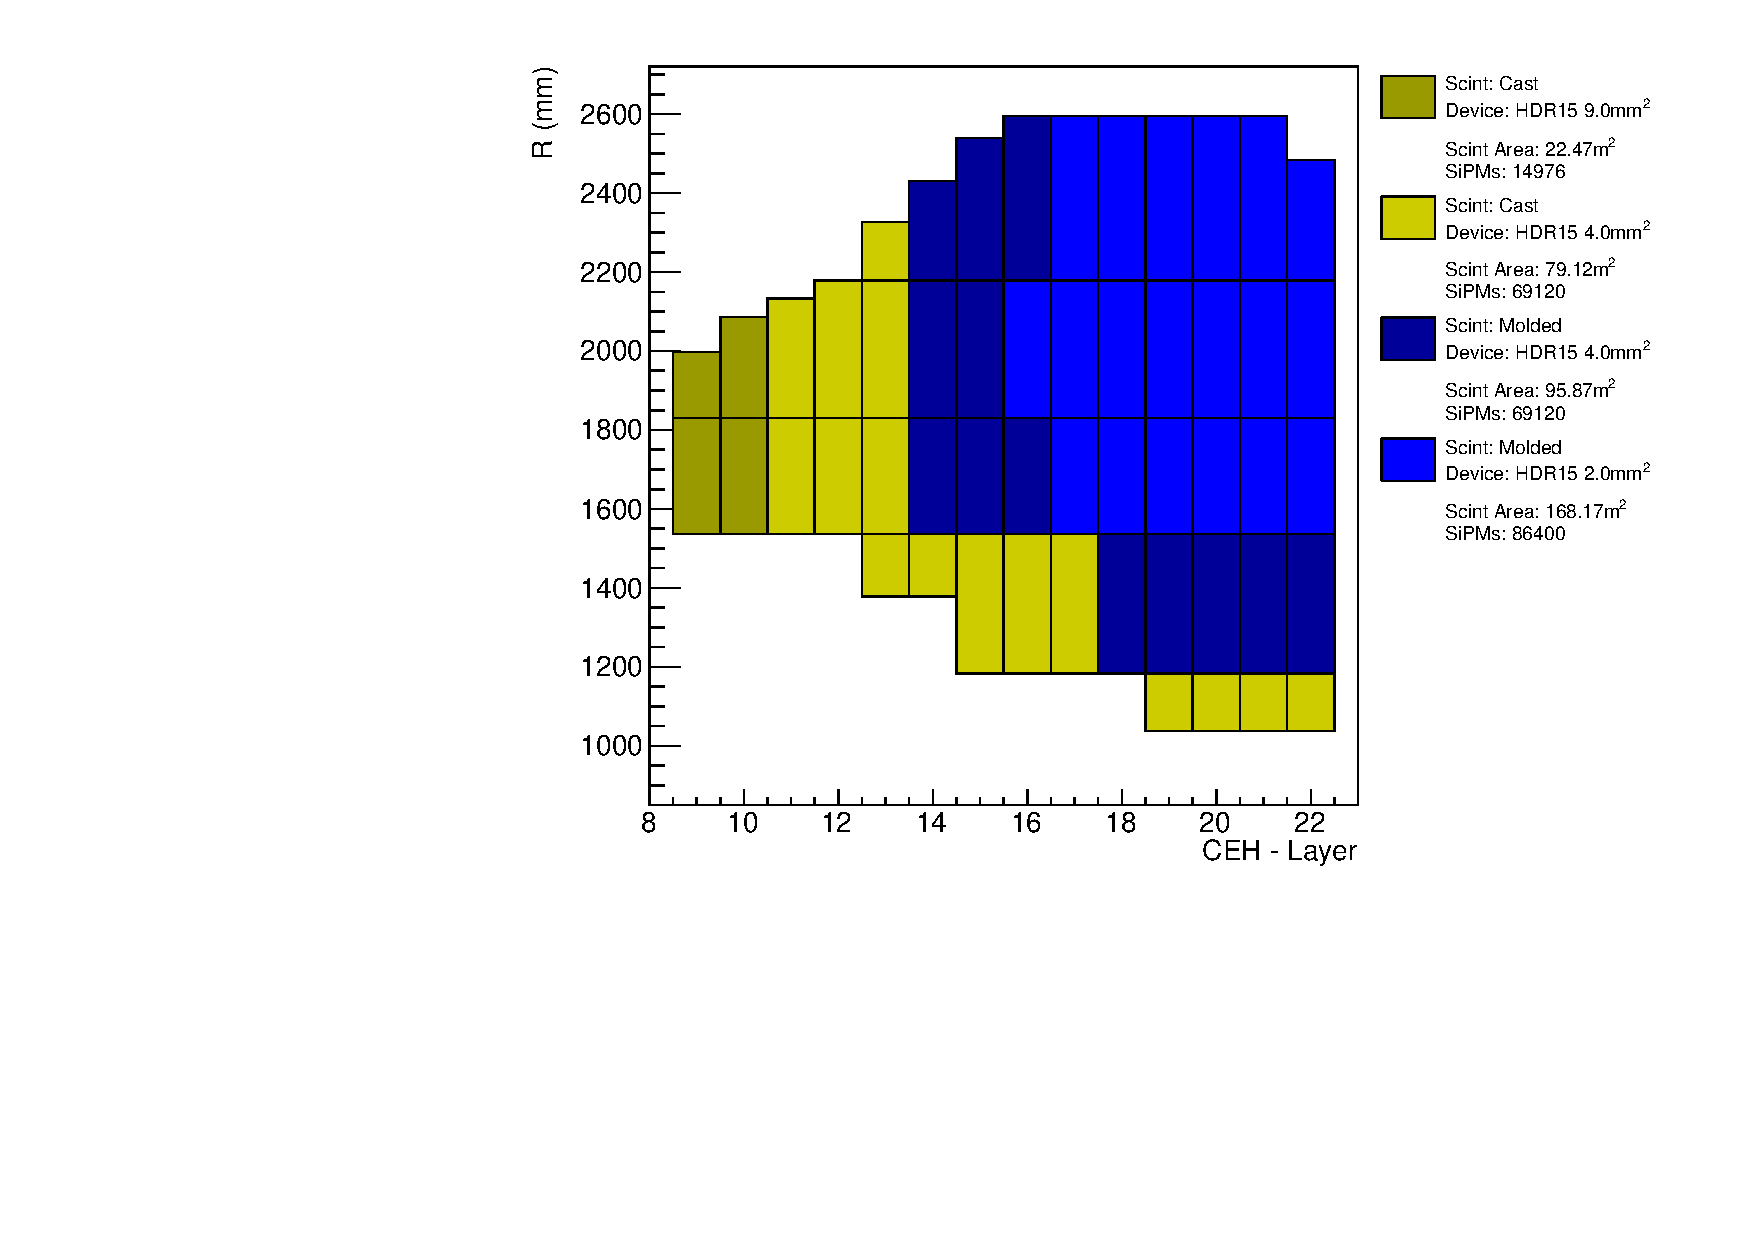
\includegraphics[trim={0 0 165pt 0},clip,width=\textwidth]{figures/hgcal/plot_scenes/sceneA_jan20_fix_vto2p0_with9mm2.pdf}
  \end{minipage}
  \begin{minipage}[c]{0.49\textwidth}
    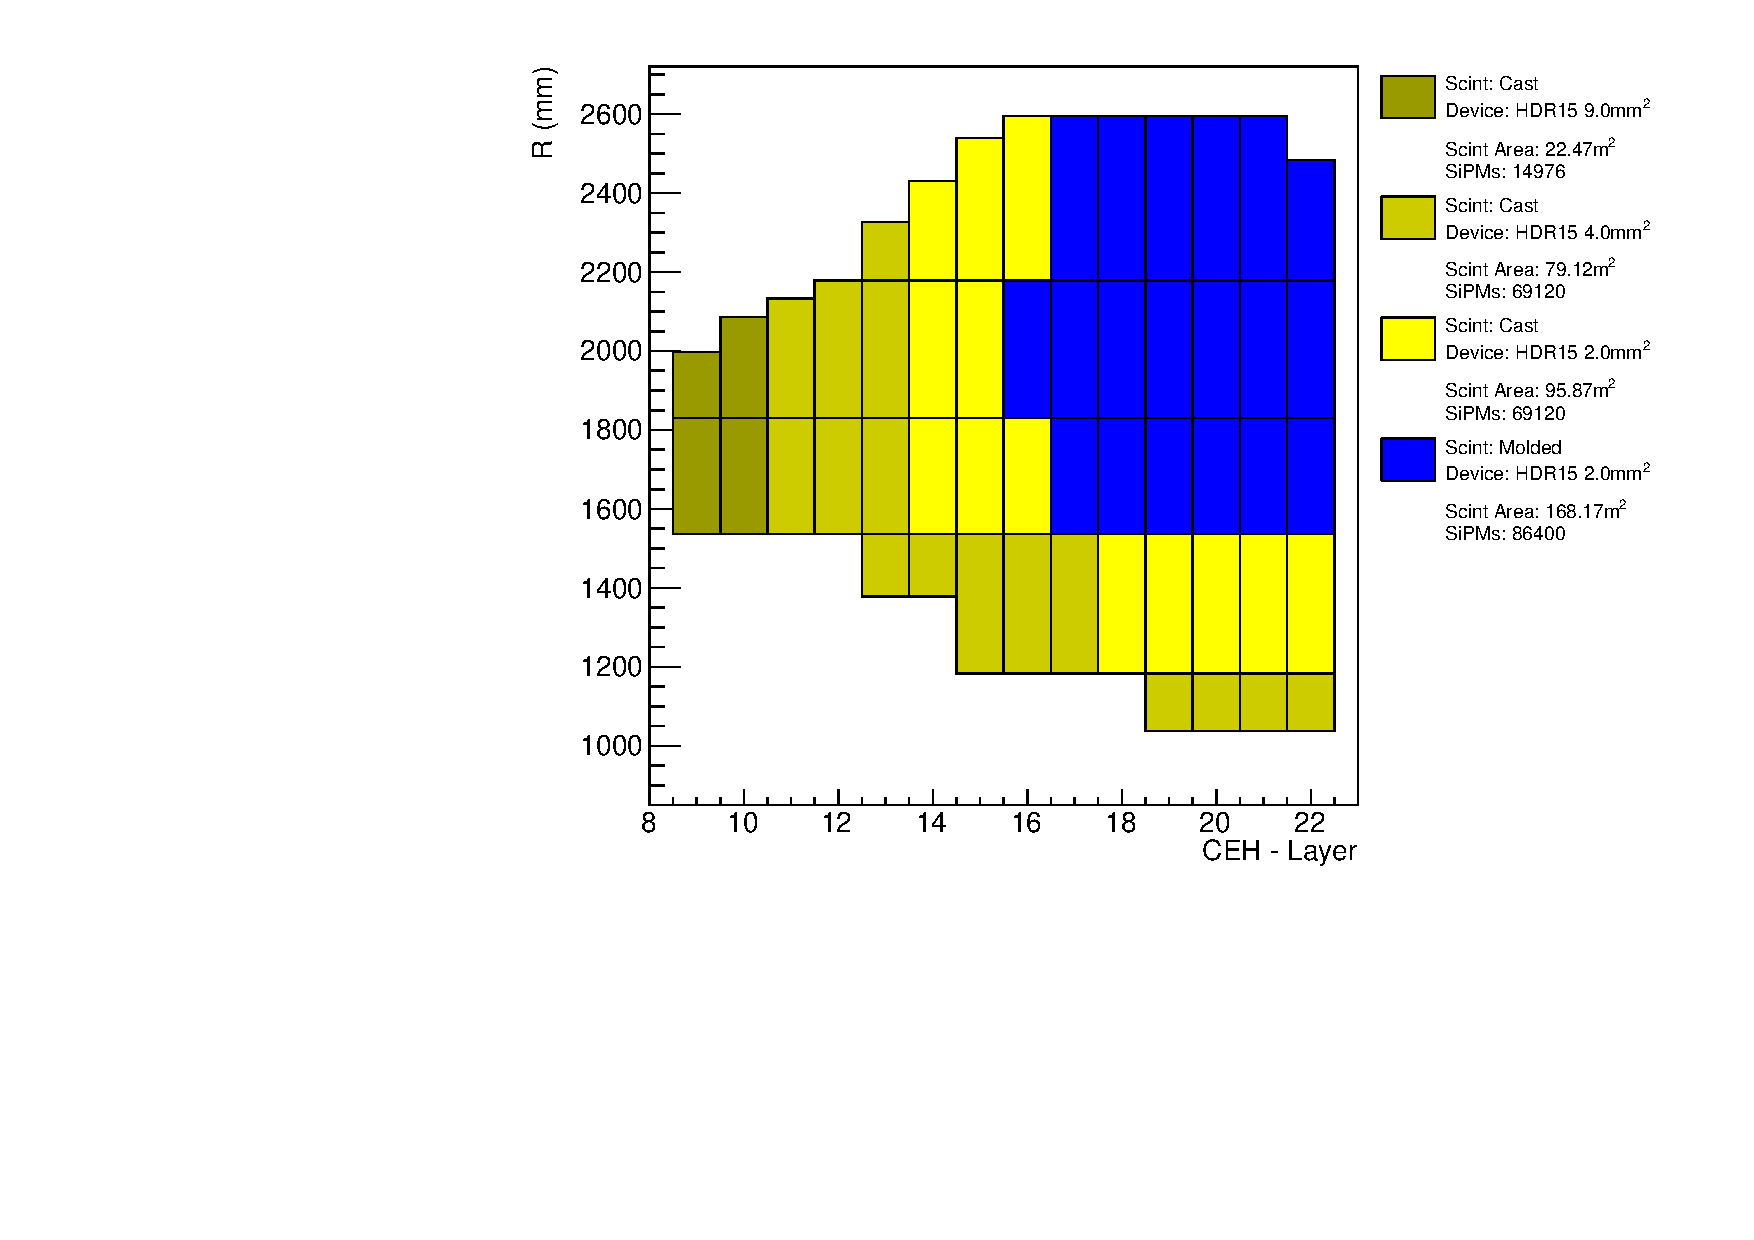
\includegraphics[trim={0 0 165pt 0},clip,width=\textwidth]{figures/hgcal/plot_scenes/sceneB_jan20_fix_vto2p0_with9mm2.pdf}
  \end{minipage}
  \caption[\gls{HGCAL} scenarios]{\gls{HGCAL} scenarios. Left: Scene A, Right: Scene B}%
  \label{fig:hgcal-scenes-fnal-jan20}
\end{figure}

\begin{table}[!ht]
  \centering
  \caption{\gls{HGCAL} scenarios comparison}\label{tab:scenarios}
  \begin{tabular}{p{1.5in}cll}%
    \toprule
                                                   &                    & Scene A                & Scene B                \\
    \midrule
    \multirow{3}{=}{Cast Scintillator}             & Cell Count         & 84, 096                & 153,216                \\
                                                   & Total Area         & 101.59 \(\text{m}^2 \) & 197.46 \(\text{m}^2 \) \\
                                                   & Percentage         & 27.8 \%                & 54.0 \%                \\
    \cmidrule(lr){2-4}
    \multirow{3}{=}{Injection Molded Scintillator} & Cell Count         & 155, 520               & 86, 400                \\
                                                   & Total Area         & 264.04 \(\text{m}^2 \) & 168.17 \(\text{m}^2 \) \\
                                                   & Percentage         & 72.2 \%                & 46.0 \%                \\
    \cmidrule(lr){2-4}
    \multirow{2}{=}{SiPMs Count}                   & 2 \(\text{mm}^2 \) & 86, 400                & 155, 520               \\
                                                   & 4 \(\text{mm}^2 \) & 138, 240               & 69, 120                \\
                                                   & 9 \(\text{mm}^2 \) & 14, 976                & 14, 976                \\
    \bottomrule
  \end{tabular}
\end{table}


Both the scenes require same number of \(9 \mm{}^{2}\) \glspl{SiPM} (Table~\ref{tab:scenarios}).
Scene B uses approximately half the \(4 \mm{}^{2}\) \glspl{SiPM}
compared to scene A. The amount of cast and injection molded
scintillator is approximately proportional in scene B. This
is beneficial to balance the tile production load between
different institutes.
For these reasons scene B is recommended to be used for \gls{HGCAL}.